% path to figures directory
\graphicspath{{img/chapter_1/}}

\chapter{Introduction}
\label{chapter:introduction}

\begin{synopsis}
  The following is a general introduction to the background topics referred to
  and assumed in subsequent chapters. This includes a review of popular theories
  of neutrino mass, the current status of neutrino-oscillation parameters, a
  general introduction to Effective Field Theory (EFT), the experimental
  situation relevant to the flavour anomalies, and topics peripheral to all of
  these.
\end{synopsis}

\section{The Standard Model and neutrinos}

Laboratory experiments to date have firmly established the predictive power of
the Standard Model (SM) of particle physics, a combined theory of the
electroweak and strong interactions described by the gauge group
$G_{\text{SM}} = \mathrm{SU}(3)_{c} \otimes \mathrm{SU}(2)_{L} \otimes \mathrm{U}(1)_{Y}$.
It is a model whose probes and predictions span at least 33 orders of
magnitude\footnote{The interval given is from the distance scales probed at the
  LHC (roughly $\SI{e-17}{\cm}$) to the size of the solar system (roughly
  \SI{e16}{\cm}).} with varying degrees of precision, and these are consistent
with almost all known experiments. Although it displays a number of arbitrary
features, the dynamics of the theory are mostly fixed by the fundamental
principles of gauge theory and Lorentz invariance. Most of this arbitrariness
resides in the matter sector of the theory, whose properties (masses, coupling
constants, quantum numbers, \textit{etc.}) are not predicted, but are instead
motivated on phenomenological grounds. We show the fields of the SM and their
defining properties in Table~\ref{tab:sm-fields}, according to the mathematical
conventions of Appendix~\ref{chapter:notation}.
\begin{table}[t]
  \centering
  \bgroup
  \def\arraystretch{1.3}% 1 is the default
  \begin{tabular}{ccc}
    \toprule
    Field                        & $\mathrm{SU}(3)_{c} \otimes \mathrm{SU}(2)_{L} \otimes \mathrm{U}(1)_{Y}$ & $\mathrm{SU}(2)_{+} \otimes \mathrm{SU}(2)_{-}$ \\
    \midrule
    $Q^{\alpha a i}$             & $(\mathbf{3}, \mathbf{2}, \tfrac{1}{6})$                                  & $(\mathbf{2}, \mathbf{1})$                      \\
    $L^{\alpha i}$               & $(\mathbf{1}, \mathbf{2}, -\tfrac{1}{2})$                                 & $(\mathbf{2}, \mathbf{1})$                      \\
    $\bar{u}^{\alpha}_a$                  & $(\bar{\mathbf{3}}, \mathbf{1}, -\tfrac{2}{3})$                           & $(\mathbf{2}, \mathbf{1})$                      \\
    $\bar{d}^{\alpha}_a$                  & $(\bar{\mathbf{3}}, \mathbf{1}, \tfrac{1}{3})$                            & $(\mathbf{2}, \mathbf{1})$                      \\
    $\bar{e}^{\alpha}$                    & $(\mathbf{1}, \mathbf{1}, 1)$                                             & $(\mathbf{2}, \mathbf{1})$                      \\
    $(G_{\alpha \beta})^a_{\ b}$ & $(\mathbf{8}, \mathbf{1}, 0)$                                             & $(\mathbf{3}, \mathbf{1})$                      \\
    $(W_{\alpha \beta})^i_{\ j}$ & $(\mathbf{1}, \mathbf{3}, 0)$                                             & $(\mathbf{3}, \mathbf{1})$                      \\
    $B_{\alpha \beta}$           & $(\mathbf{1}, \mathbf{1}, 0)$                                             & $(\mathbf{3}, \mathbf{1})$                      \\
    $H^{i}$                      & $(\mathbf{1}, \mathbf{2}, \tfrac{1}{2})$                                  & $(\mathbf{1}, \mathbf{1})$                      \\
    \bottomrule
  \end{tabular}
  \egroup
  \caption{The SM fields and their transformation properties under the SM gauge
    group $G_{\text{SM}}$ and the Lorentz group written as
    $\mathrm{SU}(2)_{+} \otimes \mathrm{SU}(2)_{-}$. The final unbolded number
    in the 3-tuples of the $G_{\text{SM}}$ column represents the
    $\mathrm{U}(1)_Y$ charge of the field, normalised such that $Q = I_{3} + Y$.
    For the fermions a generational index has been suppressed. See
    Appendix~\ref{chapter:notation} for details about the mathematical notation
    used here and throughout this work.}
  \label{tab:sm-fields}
\end{table}

The SM inherits the experimental success of the
$\mathrm{SU}(2) \otimes \mathrm{U}(1)$ theory of the weak interactions, first
proposed by Glashow~\cite{Glashow:1961tr} in 1961 as a possible underlying
structure for Fermi's theory of beta decay. Before the end of the same decade,
Weinberg~\cite{Weinberg:1967tq} and Salam~\cite{Salam:1968rm} had constructed
the modern theory of leptons based on the spontaneous breaking of
$\mathrm{SU}(2)_{L} \otimes \mathrm{U}(1)_{Y}$ to the electromagnetic symmetry.
Interestingly, it seems that these seminal papers went mostly unnoticed (see
Fig.~\ref{fig:weinberg-citations}) until the early 1970s, when 't~Hooft proved
the renormalisability of spontaneously broken gauge
theories~\cite{tHooft:1971akt} as a graduate student working under the
supervision of Veltman. By the mid 1970s the framework had been extended to
include the quarks~\cite{Glashow:1970gm} and the unbroken chromodynamic group,
which was successfully shown to reproduce the Bjorken scaling seen in
deep-inelastic-scattering experiments through asymptotic
freedom~\cite{Gross:1973id}.
\begin{figure}[t]
  \centering
  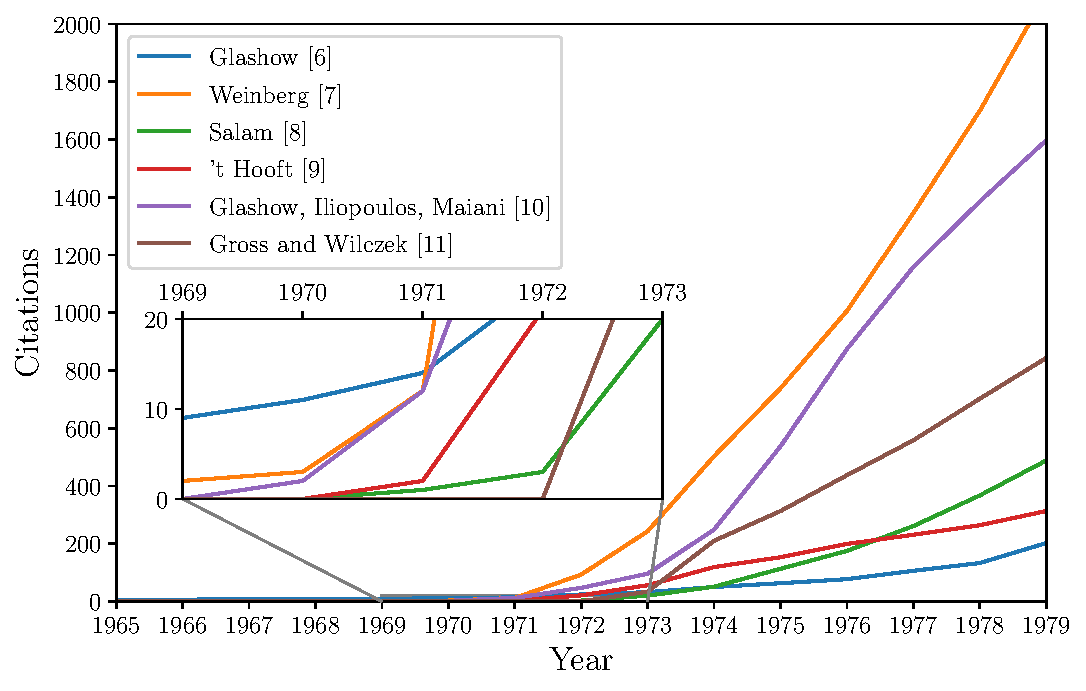
\includegraphics[width=0.9\linewidth]{weinberg_citations}
  \caption{The cumulative citation graph for a selection of papers presenting
    foundational results relevant to the SM. Weinberg's seminal paper `A model
    of leptons' (1967) saw an explosion of citations following 't~Hooft's work
    on the renormalisability of gauge theories (1971).}
  \label{fig:weinberg-citations}
\end{figure}

Despite its successes, the SM cannot be the complete theory of fundamental
particles and their interactions. It does not explain phenomena such as the
baryon asymmetry present, and the particle spectrum contains no viable candidate
for dark matter. The SM cannot explain why the electric dipole moment of the
neutron is so small, why there are three generations of matter or, notably in
our case, the origin of neutrino oscillations and the implied small but non-zero
neutrino masses.

\section{Massive neutrinos in experiment and theory}

The minimal SM predicts massless neutrinos, a prediction that today sits in
contradiction to a wealth of empirical evidence. This evidence could in
principle have come from many kinds of experiments, but currently only neutrino
oscillations provide strong signs that the masses are non-zero. Below we discuss
the phenomenon of neutrino oscillations in the context of the outstandingly
successful three-flavour mixing paradigm. We then move on to other probes of
neutrino masses, which currently only provide limits on the mass scale. On the
theory side, we summarise some popular and motivated extensions of the SM that
accommodate massive neutrinos, placing particular emphasis on the direction we
have followed in the novel work presented in this thesis. This includes an
overview of tree- and loop-level models of Majorana neutrino mass.

\subsection{Neutrino oscillations}

The neutrino flavour eigenstates $\breve{\nu}_{i}$ =
$(\nu_{e}, \nu_{\mu}, \nu_{\tau})$ are defined as the states that couple at
charged-current interaction vertices with the corresponding charged lepton.
These are the states in which the neutrinos are almost always produced in
experiments, and certainly always measured. If neutrinos are massive there is no
reason to expect these to coincide with the mass eigenstates
$\nu_{i} = (\nu_{1}, \nu_{2}, \nu_{3})$. In general, the flavour eigenstates
will be an admixture of the propagating fields
\begin{equation}
  \label{eq:neutrino-mixing}
  \breve{\nu}_{i} = U_{i}^{\ j} \nu_{j} \ ,
\end{equation}
where the $U_{i}^{\ j}$ are elements of the unitary
Pontecorvo--Maki--Nakagawa--Sakata (PMNS) neutrino mixing
matrix~\cite{Pontecorvo:1957cp, Maki:1962mu}. The PMNS matrix is defined such
that it diagonalises the neutrino mass matrix:
\begin{equation}
  \mathbf{U}^{\dagger} \mathbf{m}_{\nu} \mathbf{U}^{*} = \mathrm{diag}(m_{1}, m_{2}, m_{3}),
\end{equation}
where the $m_i$ are the neutrino masses. Being a $3 \times 3$ unitary matrix,
$\mathbf{U}$ is in general parametrised by three mixing angles and six phases.
Not all of the phases are physical, since the neutrino and charged-lepton fields
can be redefined in such a way that five of the phases are removed in the case
of Dirac neutrinos. In the presence of a Majorana mass term, only the charged
leptons can be rephased. This leaves three physical phases with the two
additional ones termed \textit{Majorana phases}. In general
\begin{equation}
  \label{eq:pmns}
  \mathbf{U} =
  \begin{bmatrix}
    c_{12}c_{13} & s_{12} c_{13} & s_{13}e^{-i\delta_\text{CP}} \\
    -s_{12}c_{23} - c_{12}s_{23}s_{13}e^{i\delta_\text{CP}} & c_{12}c_{23} - s_{12}s_{23}s_{13}e^{i\delta_\text{CP}} & s_{23}c_{13}\\
    s_{12}s_{23} - c_{12}c_{23}s_{13}e^{i\delta_\text{CP}} & -c_{12}s_{23} - s_{12}c_{23}s_{13}e^{i\delta_\text{CP}} & c_{23}c_{13}
  \end{bmatrix}
  \mathbf{P} \ ,
\end{equation}
where $c_{ij} = \cos \theta_{ij}$, $s_{ij} = \sin \theta_{ij}$ and
\begin{equation}
  \mathbf{P} =
  \begin{cases}
    \mathrm{diag}(e^{i \alpha_{1}}, e^{i \alpha_{2}}, 1) & \text{for Majorana neutrinos} \\
    \mathbf{1}_{3 \times 3} & \text{for Dirac neutrinos} \\
  \end{cases} \ .
\end{equation}
The phase $\delta_{\text{CP}}$ is often called the \textit{Dirac phase}, while
$\alpha_{1,2}$ are the Majorana phases discussed above.

Neutrino oscillation experiments typically involve the production of neutrino
flavour states from charged-current processes, \textit{e.g.} leptonic pion
decays. Each mass eigenstate evolves in time independently according to the
Schr\"{o}dinger equation: \textit{i.e.}
$| \nu_{i} (t) \rangle = \exp{(-i E_{i} t)} | \nu_{i} (0) \rangle$, for evolution
\textit{in vacuo}. This alters the initial superposition away from being a pure
flavour eigenstate:
\begin{align}
  | \breve{\nu}_{i} (t) \rangle &= \sum_{j} U_{i}^{* j} e^{-i E_{j} t} | \nu_{j} \rangle \\
                                &= \sum_{j,k} U_{i}^{* j} e^{-i E_{j} t} U_{j}^{\ k} | \breve{\nu}_{k} \rangle \ .
\end{align}
The probability of measuring a specific flavour through the charged-current
interaction then oscillates with time:
\begin{equation}
  \text{P}(\breve{\nu}_{m} \to \breve{\nu}_{n}) = | \langle \breve{\nu}_{n} | \breve{\nu}_{m} (t) \rangle |^{2} = \left| \sum_{i} U_{m}^{* i} U_{i}^{\ n} e^{-i E_{i} t} \right|^{2} \ .
\end{equation}
The expression can be expanded and the kinematic factors simplified from the
fact that the neutrinos are ultra-relativistic. We follow the usual convention
and take
$E_{i} = \sqrt{\mathbf{p}^{2} + m_{i}^{2}} \approx |\mathbf{p}| + m_{i}^{2} / (2 E)$
with $E = |\mathbf{p}|$. This gives
\begin{equation}
  \label{eq:neutrino-osc}
  \begin{aligned}
    \text{P}(\breve{\nu}_{m} \to \breve{\nu}_{n}) &= \delta_{mn} - 4 \sum_{i < j} \mathrm{Re}\left( U_{m}^{\ i} U_{m}^{* j} U_{n}^{* i} U_{n}^{\ j}  \right) \sin^{2} \frac{\Delta m_{ij}^{2} L}{4E}\\
    &\quad + 2 \sum_{i<j} \mathrm{Im}\left( U_{m}^{\ i} U_{m}^{* j} U_{n}^{* i} U_{n}^{\ j}  \right) \sin \frac{\Delta m^{2}_{ji} L}{2E} \ ,
  \end{aligned}
\end{equation}
where $\Delta m_{ij}^{2} \equiv m_{j}^{2} - m_{i}^{2}$ are the squared neutrino
mass differences and $L = ct$, sometimes called the baseline, is the approximate
distance travelled by the particles. To interpret the results of many
experiments, it is often sufficient to consider an effective two-flavour
oscillation paradigm. In this case, the neutrino-oscillation probabilities are
governed by by a single squared mass difference $\Delta m^{2}$ and a single
angle $\theta$. Interestingly, the CP-violating phase is completely absent from
the two flavour formula:
\begin{equation}
  \label{eq:two-flavour-osc}
  \text{P}(\breve{\nu}_{m} \to \breve{\nu}_{n})_{n_{f}=2} = \sin^{2} (2\theta) \sin^{2} \frac{\Delta m^{2} L}{4E} \ .
\end{equation}

From the expressions in Eqs.~\eqref{eq:neutrino-osc} and
\eqref{eq:two-flavour-osc} a number of properties of the vacuum neutrino
oscillations become clear.
\begin{enumerate}
  \item The neutrino oscillation probabilities depend on the neutrino mass
    differences, and not on the absolute mass scale. For three flavours, there
    are only two independent squared mass differences. Typically chosen to be
    $\Delta m_{21}^{2}$ and $\Delta m_{31}^{2}$, although often they are
    refereed to with the historical names $\Delta m_{\text{sol}}^{2}$ and
    $\Delta m_{\text{atm}}^{2}$, discussed in detail below.
  \item From Eq.~\eqref{eq:neutrino-osc} it is clear that the oscillations only
    occur if the neutrinos are non-degenerate and the neutrino mixing is
    non-trivial, \textit{i.e.} if $\Delta m_{ij} \neq 0$ and
    $\mathbf{U} \neq \mathbf{1}$.
  \item The PMNS matrix elements only appear in the combination
    $U_{m}^{\ i} U_{m}^{* j}$, to which the Majorana phases contained within the
    matrix $\mathbf{P}$ do not contribute. This implies that oscillation
    experiments cannot comment on the Dirac or Majorana nature\footnote{Of
    course, this is already clear from the fact that neutrino oscillations
    conserve total lepton number, despite breaking the individual familial
    lepton-number symmetries $L_{e, \mu, \tau}$.} of the neutrinos. Oscillations
    can however probe $\delta_{\text{CP}}$.
  \item In the effective two-flavour mixing paradigm, both $\theta$ and
    $\Delta m^{2}$ appear in such a way that neither the sign of $\Delta m^{2}$
    nor the octant of $\theta$ can be uniquely determined.
  \end{enumerate}
  Thus, neutrino oscillations imply that the neutrino masses of at least two of
  the mass eigenstates are non-degenerate, and therefore only one neutrino could
  potentially be massless. The largest squared mass difference can therefore be
  translated into an lower bound on the mass of the heaviest neutrino, which we
  present later with modern data.

  Historically, the effective two-flavour mixing paradigm has provided a good
  framework for interpreting early indications of neutrino oscillations.
  Specifically, the solar and atmospheric neutrino puzzles have approximate
  descriptions in terms of a two-flavour picture. Oscillations
  $\nu_{e} \to \nu_{\text{active}}$, where $\nu_{\text{active}}$ is a coherent
  superposition of $\nu_{\mu}$ and $\nu_{\tau}$, in both matter and vacuum
  account for the deficit of electron neutrinos measured from the sun, and
  $\nu_{\mu} \to \nu_{\tau}$ oscillations \textit{in vacuo} explain the shortage
  of muon neutrinos from cosmic-ray-induced production in the upper atmosphere.

  The measurement and resolution of these puzzles is an interesting and exciting
  chapter in the recent history of physics. Experiments as early as the 1960s
  had noticed a shortage of electron neutrinos coming from the sun relative to
  the predictions of solar models~\cite{RevModPhys.60.297, 1988ApJ...335..415T,
    RevModPhys.64.885, RevModPhys.67.781}, which themselves were subject to much
  uncertainty~\cite{Morrison:1992bz}. For detection there were three main
  approaches: Raymond Davis and collaborators~\cite{PhysRevLett.12.303}
  pioneered experiments that measured the solar electron-neutrino flux using
  Chlorine, the Kamiokande and later Super-Kamiokande
  collaborations~\cite{Hirata:1989zj, Hirata:1990xa} used water Cherenkov
  detectors, and the experiments GALLEX~\cite{Hampel:1998xg} and
  SAGE~\cite{Abdurashitov:1999zd} had Gallium as the detecting material. All of
  these experiments showed a deficit of solar electron neutrinos, although they
  were sensitive to neutrinos of different energies. The Sudbury Neutrino
  Observatory gave the final word on the oscillation solution to the solar
  neutrino puzzle with accurate confirmation of the electron-neutrino deficit,
  along with a measurement of the \textit{total} neutrino flux which was found
  to be in agreement with the solar models~\cite{Ahmad:2001an, Ahmad:2002jz}.

  Atmospheric neutrinos were known to come about from helicity-suppressed kaon
  and pion decays to muons and muon neutrinos. A zenith-angle and
  energy-dependent suppression in the flux of atmospheric muon neutrinos was
  measured by the Kamiokande and Irvine--Michigan--Brookhaven
  experiments~\cite{Hirata:1992ku, BeckerSzendy:1995vr} in the early 1990s, and
  after the upgrade to Super-Kamiokande the deficit was confirmed to high
  precision with results presented at the `Neutrino 1998'
  conference~\cite{Fukuda:1998mi, vonFeilitzsch:2003mh, shiozawa:2002,
    Smy:2002rz}.

  The pairs of mixing parameters associated with these two classes of
  measurements are usually dubbed
  $\theta_{\text{sol}}, \Delta m^{2}_{\text{sol}}$ and
  $\theta_{\text{atm}}, \Delta m^{2}_{\text{atm}}$. Experimental results find
  $\Delta m^{2}_{\text{sol}} \ll \Delta m^{2}_{\text{atm}}$ and that both
  $\theta_{\text{sol}}$ and $\theta_{\text{atm}}$ are large compared to any
  angles found in the CKM matrix, the quark mixing matrix. Interpreted in terms
  of three-flavour mixing, common convention identifies
  $\Delta m_{\text{sol}}^{2}$ with the squared mass difference between $\nu_{2}$
  and $\nu_{1}$, which is known to be positive\footnote{We note that the sign of
    $\Delta m_{21}^{2}$ can be known since oscillations in matter are also
    relevant for the solar squared mass difference, which depart from the simple
    formula of Eq.~\eqref{eq:two-flavour-osc}.} (\textit{i.e.}
  $\Delta m^{2}_{21} > 0$). The solar mixing angle $\theta_{\text{sol}}$ is then
  associated with $\theta_{12}$. The atmospheric mixing parameters are
  identified with $|\Delta m_{31}^{2}|$ or $|\Delta m_{32}^{2}|$ and
  $\theta_{23}$. Of course, three-flavour effects alter the simplistic picture
  presented here and must be included to interpret measurements of $\theta_{13}$
  and $\delta_{\text{CP}}$, see \textit{e.g.} Ref.~\cite{Giganti:2017fhf} and
  references therein for a more detailed discussion. The picture that emerges
  from these experiments is then
  \begin{equation}
    \Delta m^{2}_{\text{sol}} \approx \Delta m^{2}_{21} \ll |\Delta m_{31}^{2}| \approx |\Delta m_{32}^{2}| \approx |\Delta m_{\text{atm}}^{2}| \ ,
  \end{equation}
  with which both the \textit{normal mass ordering} $m_{1} < m_{2} < m_{3}$ and
  the \textit{inverted mass ordering} $m_{3} < m_{1} < m_{2}$ are consistent.

  Neutrino oscillation experiments have continued to probe the squared mass
  differences and mixing parameters with impressively high precision, see
  \textit{e.g.} Refs.~\cite{Capozzi:2017ipn, Esteban:2020cvm}. Reactor neutrino
  experiments like KamLAND~\cite{Eguchi:2002dm} and long-baseline accelerators,
  \textit{e.g.} T2K~\cite{Abe:2015awa} and NO$\nu$A~\cite{Adamson:2017qqn}, are
  sensitive to all of these parameters, although $\Delta m^{2}_{\text{atm}}$ and
  $\theta_{13}$ are best measured at short-baseline reactors like Double
  Chooz~\cite{Ardellier:2006mn}, RENO~\cite{Ahn:2010vy} and Daya
  Bay~\cite{An:2015qga}. Today the octant of $\theta_{12}$ is certainly known,
  while $\theta_{13}$ is constrained to be close to 0.15. The sign of the
  atmospheric squared mass difference is still unknown, and therefore so is the
  mass ordering for the neutrinos. The value of the CP-violating Dirac phase
  $\delta_{\text{CP}}$ is less clear, although there is a preference for a value
  somewhere between $\pi$ and $3\pi/2$. The extent of CP-violation in the
  neutrino sector can be represented in a rephasing-invariant way with the
  leptonic Jarlskog invariant
  \begin{equation}
    J_{CP} = \frac{1}{8} \cos \theta_{13} \sin 2\theta_{12} \sin 2\theta_{13} \sin 2\theta_{23} \sin \delta_{\text{CP}} \ ,
  \end{equation}
  so a value of $\pi$ would imply no CP-violating effects, while
  $\delta_{\text{CP}} = 3\pi/2$ would make these maximal. For this work we take
  the results of the most recent fit to neutrino oscillation data by the NuFit
  collaboration~\cite{Esteban:2020cvm, nufitweb} in the context of the
  three-flavour paradigm. These results are summarised in
  Fig.~\ref{fig:nufit-results} separately for the cases of normal and inverted
  mass ordering. Results including atmospheric neutrino oscillation data from
  Super-Kamiokande and those not are also distinguished. Two-dimensional
  projections of the $\chi^{2}$ fit for the same parameters are shown in
  Fig.~\ref{fig:nufit-2d-results}. These data suggest a leptonic mixing matrix
  that has a very different form to the CKM matrix, which we call $\mathbf{V}$.
  We represent this qualitatively by using boxes whose side lengths are scaled
  to the magnitude of the best-fit values of the parameters in the matrices, the
  textures are
  \begin{equation}
    \label{eq:pmns-ckm-comparison}
    \mathbf{U} \sim
    \begin{pmatrix}
       \rule{0.825146em}{0.825146em} & \rule{0.544911em}{0.544911em} & \rule{0.149018em}{0.149018em} \\
       \rule{0.271967em}{0.271967em} & \rule{0.607533em}{0.607533em} & \rule{0.746283em}{0.746283em} \\
       \rule{0.440837em}{0.440837em} & \rule{0.577907em}{0.577907em} & \rule{0.648734em}{0.648734em} \\
     \end{pmatrix}, \qquad
     \mathbf{V} \sim
     \begin{pmatrix}
       \rule{0.97427em}{0.97427em}  & \rule{0.22534em}{0.22534em} & \rule{0.00351em}{0.00351em} \\
       \rule{0.22520em}{0.22520em}  & \rule{0.97344em}{0.97344em} & \rule{0.0412em}{0.0412em} \\
       \rule{0.00867em}{0.00867em}  & \rule{0.0404em}{0.0404em} & \rule{0.999146em}{0.999146em} \\
     \end{pmatrix} \ .
  \end{equation}
  For the PMNS matrix we take the best fit values for the normal mass ordering
  including the Super-Kamiokande results, \textit{i.e.} the numbers in the
  top-left quadrant of Fig.~\ref{fig:nufit-results}. The same numbers also imply
  an upper bound on the mass of the heaviest neutrino at
  \begin{equation}
    \label{eq:atmospheric-bound}
    m_{\text{heaviest}} \leq \sqrt{|\Delta m_{\text{atm}}^{2}|} \approx \SI{0.05}{\eV} \ .
  \end{equation}

  \begin{figure}
    \centering
    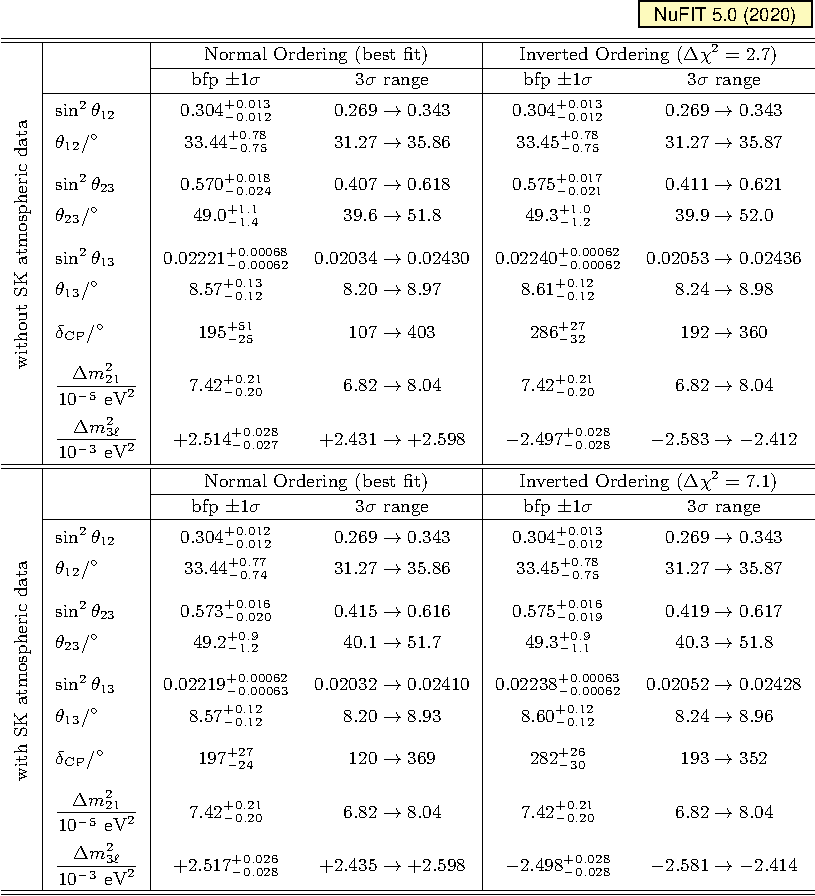
\includegraphics[width=0.9\linewidth]{v50.tbl-parameters}
    \caption{The figure shows a table taken from the latest global fit to
      neutrino mass and mixing parameters by the NuFit
      collaboration~\cite{Esteban:2020cvm, nufitweb} in the three-flavour
      picture. The results presented in the upper (lower) panel are obtained by
      excluding (including) the $\chi^{2}$ data on atmospheric neutrinos
      provided by the Super-Kamiokande collaboration (SK). The numbers in the
      1st (2nd) column are obtained assuming normal (inverted) neutrino mass
      ordering. See Ref.~\cite{nufitweb} for more information.}
    \label{fig:nufit-results}
  \end{figure}
 
  \begin{figure}
    \centering
    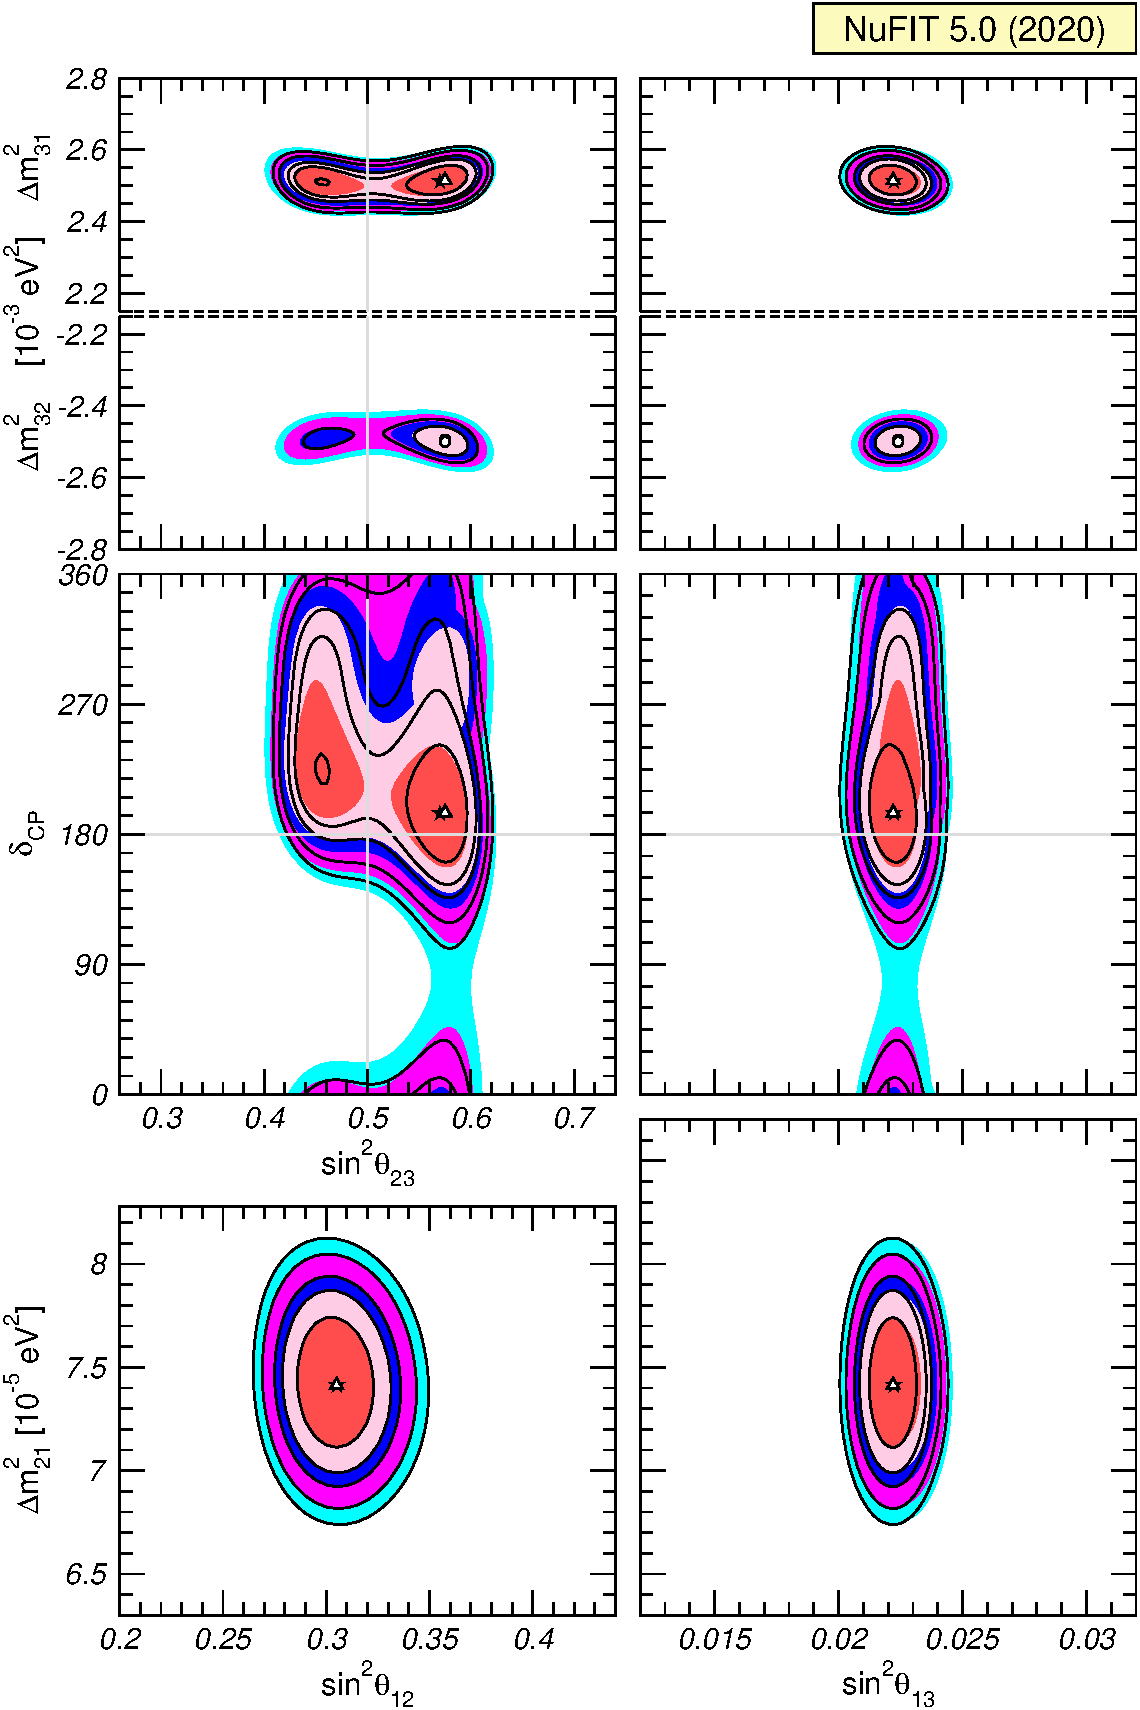
\includegraphics[width=0.8\linewidth]{v50.fig-region-glob}
    \caption{The figure shows the two-dimensional allowed regions obtained by
      the latest fit to the neutrino mass and mixing parameters by the NuFit
      collaboration~\cite{Esteban:2020cvm, nufitweb}. Each plot shows the
      two-dimensional projection of the allowed region after marginalising with
      respect to the other parameters. The coloured regions (black contour
      curves) are obtained by excluding (including) the Super-Kamiomande
      $\chi^{2}$ data. The different contours correspond to the two-dimensional
      allowed regions at $1\sigma$, $90\%$, $2\sigma$, $99\%$, $3\sigma$
      confidence. See Ref.~\cite{nufitweb} for more information.}
    \label{fig:nufit-2d-results}
  \end{figure}

\subsection{Other experimental probes}

Although neutrino oscillations provide a wealth of evidence for non-zero masses
for at least two of the neutrino fields, they do not probe the absolute mass
scale. There are however kinematic and cosmological probes which bound the
neutrino masses, and some of these are mentioned here.

\subsubsection{Beta decay}

A study of the kinematics of beta-decay experiments shows that differences in
the energy distribution of the emitted electron are expected for different
values of the neutrino mass. Currently these experiments only provide upper
bounds on the effective neutrino mass~\cite{Shrock:1980vy}
\begin{equation}
  m_{\beta} \equiv \sqrt{\sum_{i} |U_{1}^{\ i}|^{2} m_{i}^{2}} \ .
\end{equation}
The best results come from tritium experiments which probe
${}^{3}\mathrm{H} \to {}^{3}\mathrm{He} + e + \bar{\nu}_{e}$. The KATRIN
experiment recently presented the most stringent upper bound~\cite{Aker:2019uuj,
  Aker:2019qfn}
\begin{equation}
  \label{eq:2}
  m_{\beta} < \SI{1.1}{\eV} \ ,
\end{equation}
at $90\%$ confidence, with a projected limit of $m_{\beta} < \SI{0.2}{\eV}$ with
the full dataset.

Another process with the potential to probe the absolute scale of the neutrino
masses, as well as the Majorana phases, is neutrinoless double beta decay
($0\nu\beta\beta$). The process requires the violation of lepton-number by two
units, and is therefore intimately tied to the neutrinos' possible Majorana
nature. If double-beta decay is seen, the \textit{black box
  theorem}~\cite{Schechter:1981bd, Takasugi:1984xr, Hirsch:2006yk} guarantees
that the neutrinos pick up a radiative Majorana mass, even if the neutrino
masses vanish at tree level. Graphically this is easy to understand: a
$0\nu\beta\beta$ operator can always be turned into a neutrino self-energy graph
with four loops. The amplitude for the process is proportional to
\begin{equation}
  \langle m_{\nu} \rangle_{\beta\beta} = \sum_{i} (U_{1}^{\ i})^{2} m_{i} \ ,
\end{equation}
which features both the neutrino masses and the Majorana phases. (Of course it
may be that the four-loop contribution to the neutrino mass implied by the
double-beta-decay operator represents only a small correction to the neutrino
masses, which could arise at lower order.) Current limits on
$\langle m_{\nu} \rangle_{\beta\beta}$ are around \SI{0.2}{\eV}, see
\textit{e.g.} Ref.~\cite{Dolinski:2019nrj} for a recent review of the
experimental status and prospects. Constraints on
$\langle m_{\nu} \rangle_{\beta\beta}$ are usually presented against the mass of
the lightest neutrino mass eigenstate. The behaviour of
$\langle m_{\nu} \rangle_{\beta\beta}$ is very sensitive to the neutrino mass
ordering, in such a way that the inverted scenario implies a minimum allowed
value of $\langle m_{\nu} \rangle_{\beta\beta}$, which will begin to be probed
by the next generation of experiments. A combined global limit and the projected
sensitivity of the DARWIN experiment~\cite{Agostini:2020adk} are shown in
Fig.~\ref{fig:0vbb-darwin}, which also illustrates the different behaviour of
the inverted and normal neutrino mass orderings in the
$\langle m_{\nu} \rangle_{\beta\beta}$ vs. $m_{\text{lightest}}$ plane.

\begin{figure}[t]
  \centering
  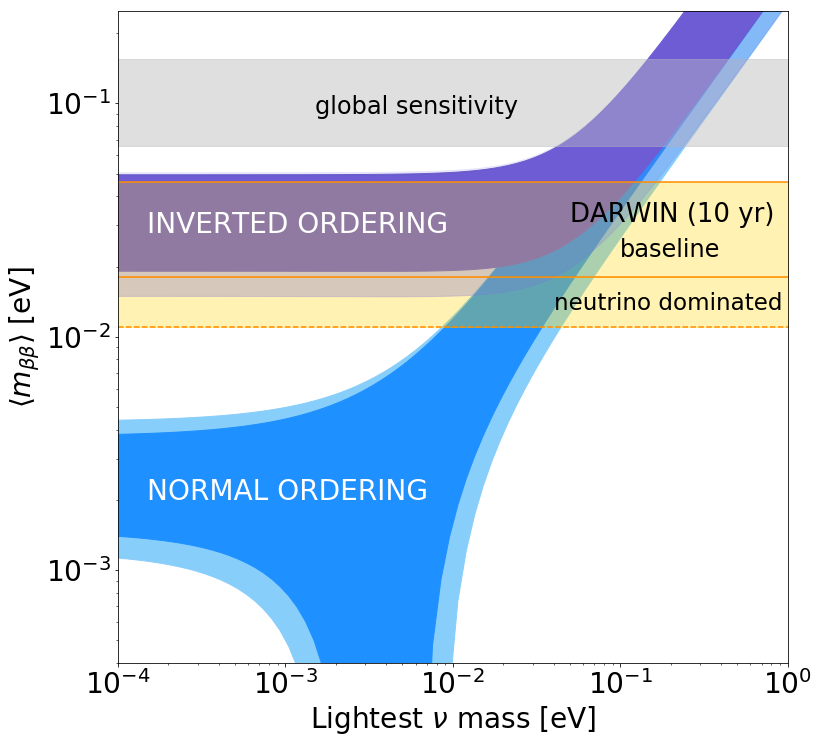
\includegraphics[width=0.6\linewidth]{0vbb_darwin}
  \caption{The figure shows limits on the effective neutrino mass for different
    values of $m_{\text{lightest}}$ for both normal and inverted mass ordering.
    The grey region represents the combined sensitivity from a number of leading
    experiments~\cite{Agostini:2019hzm}. The yellow regions are projections for
    the DARWIN experiment under different background hypotheses. The figure is
    taken from Ref.~\cite{Agostini:2020adk}, and we point the reader there for
    more information.}
  \label{fig:0vbb-darwin}
\end{figure}

\subsubsection{Cosmological limits}

The most stringent limits on the sum of the neutrino masses come from cosmology,
although they are model-dependent. In the minimal $\Lambda$CDM model adjusted
for massive neutrinos, the limit implied by the most recent Planck data
release~\cite{Aghanim:2018eyx} is
\begin{equation}
  \sum_{i} m_{i} < \SI{0.12}{\eV} \ ,
\end{equation}
at $95\%$ confidence. This is impressively small, and puts pressure on the
inverted-ordering scenario, for which $\sum_{i} m_{i} \gtrsim \SI{0.1}{\eV}$.
Excitingly, future cosmological probes will likely make a measurement of the sum
of the neutrino masses.

\subsection{Models of neutrino masses}
\label{sec:ch1-models-of-mv}

In the SM the neutrino fields appear only within the lepton doublet $L$, and one
cannot write down---in analogy to the up-type Yukawa---a renormalisable operator
that leads to neutrino masses because of the absence of the right-handed fields.
A simple model of neutrino mass then involves introducing right-handed neutrino
fields $\bar{\nu} \sim (\mathbf{1}, \mathbf{1}, 0)_{(\mathbf{1}, \mathbf{2})}$,
extending the Yukawa sector of the SM accordingly to
\begin{equation}
  -\mathscr{L}_{Y} \supset y_{e}\bar{e}LH^{\dagger} + y_{d}\bar{d}QH^{\dagger} + y_{u} \bar{u}QH + y_{\nu}\bar{\nu}LH \ ,
\end{equation}
in a simplified one-flavour picture. This implies Dirac neutrinos with a mass
$m_{\nu} \approx y_{\nu} v$, and makes mass generation symmetric between the
quarks and leptons.

There are a number of problems with this simplistic scenario. First, it is
perhaps uncomfortable to suppose that the neutrinos are many orders of magnitude
lighter than the charged fermions only because $y_{\nu}$ is a very small number.
Indeed, the posited large hierarchy between $y_{\nu}$ and $y_{u}$ seems to spoil
any aesthetic arguments for quark--lepton symmetry in favour of this hypothesis.
Although the Yukawa couplings for the other SM fermions span six orders of
magnitude, couplings within any one generation are all of similar order. We
illustrate this in Fig.~\ref{fig:fermion-masses}, where the fermion masses are
plotted by generation. Whereas one could consider that some underlying theory of
flavour may explain, for example, the disparity in scale between the masses of
the electron and the top quark, the large mass difference between the electron
and the lightest neutrino, although technically natural, seems to cry out for
its own explanation.

A second point of criticism with the simple scenario presented above is that it
ignores the Majorana mass term for $\bar{\nu}$
\begin{equation}
  \label{eq:3}
  \mathscr{L} \supset - \tfrac{1}{2} \mu \bar{\nu} \bar{\nu} + \text{h.c.}
\end{equation}
In order to maintain the Dirac neutrino mass with the relation
$m_{\nu} \approx y_{\nu}v$, the Majorana mass must be forbidden or else chosen
to be negligibly small, assumptions adding additional layers of contrivance to
the theory. A sensible choice for the scale $\mu$ is some high scale $\Lambda$
associated with the breaking of $\mathrm{U}(1)_{B-L}$. Taking
$\mu \gg y_{\nu} v$, the neutrino-mass matrix takes on the form
\begin{equation}
  \mathbf{m}_{\nu} = \begin{pmatrix}
    0 & y_{\nu} v \\
    y_{\nu} v & \mu \\
  \end{pmatrix} \ ,
\end{equation}
with eigenvalues
\begin{equation}
  m_{l} \approx \frac{y_{\nu}^{2}v^{2}}{\mu},\quad m_{h} \approx \mu \ .
\end{equation}
The assumption $\mu \gg y_{\nu} v$ implies that $m_{l} \ll y_{\nu} v$, and the
neutrino is successfully arranged to be much lighter than $y_{\nu} v$, which can
now be taken to be on the order of the charged fermion masses. The theory also
leaves us with a neutrino whose mass must be significantly larger than the
electroweak scale: $m_{h} \gtrsim \SI{e14}{\GeV}$, assuming
$m_{l} = \SI{0.05}{\eV}$ and $y_{\nu} = 1$. After transforming into the
mass-diagonal basis, the physical fields $\nu_{l}$ and $\nu_{h}$ correspond to
Majorana particles. Thus, in the most motivated region of parameter space, the
phenomenology of the light neutrinos in even the $\text{SM} + \bar{\nu}$
scenario is Majorana. This toy scenario illustrates the mechanism commonly
called the \textit{seesaw mechanism}: making the neutrinos very light at the
expense of making other fields very heavy. This is discussed more broadly below.

\begin{figure}[t]
  \centering
  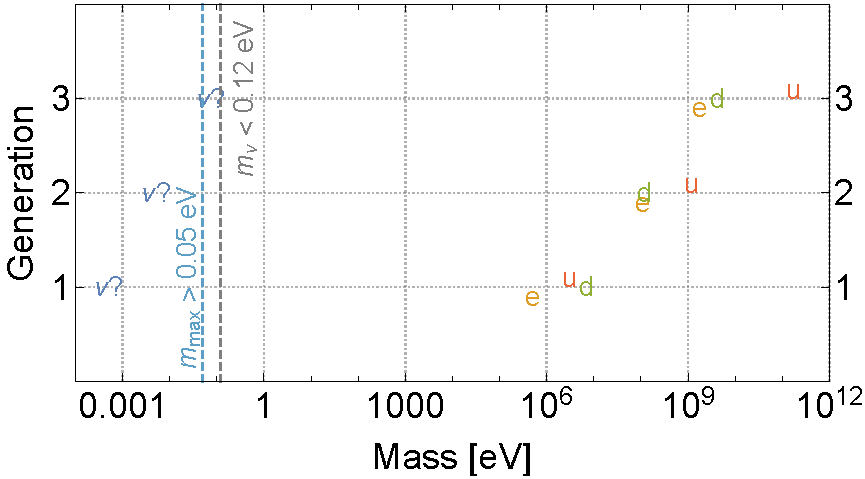
\includegraphics[width=0.7\linewidth]{fermion_mass_plot}
  \caption{The masses of the SM fermions grouped by generation. While the SM
    Yukawa couplings span a wide range of values, within any specific generation
    they are all of similar order. The tiny masses of the neutrinos seem to
    suggest an alternate mass-generation mechanism.}
  \label{fig:fermion-masses}
\end{figure}

\subsubsection{Tree-level models of neutrino mass}

The toy seesaw scenario discussed above can be understood more generally by
studying the effective theory valid below the scale $\mu$, which does not
contain the field $\bar{\nu}$. The leading-order lepton-number-violating (LNV)
effects appear at dimension five in the operator
\begin{equation}
  \mathscr{L} \supset \frac{\kappa}{\Lambda} (L^{i}L^{j})H^{k}H^{l} \cdot \epsilon_{ik}\epsilon_{jl} \ ,
\end{equation}
with $\kappa$ a dimensionless coefficient. This operator is commonly called the
\textit{Weinberg operator}. In the broken phase it gives rise to a Majorana mass
for the neutrinos consistent with the seesaw formula:
\begin{equation}
  \label{eq:seesaw-formula}
  \mathscr{L} \supset \frac{v^{2} \kappa}{\Lambda} \nu \nu \ .
\end{equation}

The $\text{SM}+\bar{\nu}$ scenario is not the only simplified model that
generates the Weinberg operator at tree-level. A simple diagram-topology
analysis suggests there are another two seesaw mechanisms in the UV: a model
with a scalar isotriplet field $\Xi_{1} \sim (\mathbf{1}, \mathbf{3}, 1)_{S}$,
called the type-II mechanism, and another with an isotriplet Majorana fermion
$\Sigma \sim (\mathbf{1}, \mathbf{3}, 0)_{F}$, called type-III. Along with the
type-I heavy $\bar{\nu}$ model, these are collectively referred to as the
canonical seesaw mechanisms~\cite{MINKOWSKI1977421, Yanagida:1979as,
  GellMann:1980vs, PhysRevLett.44.912, Glashow:1979nm, Magg:1980ut,
  PhysRevD.22.2227, LAZARIDES1981287, Wetterich:1981bx, PhysRevD.23.165,
  Foot:1988aq} and have been studied at length in the literature. They are
simple models in that they introduce only very few exotic degrees of freedom and
free parameters. However, the high seesaw scale makes these models practically
untestable at current and future collider experiments.

Models of Majorana neutrino mass can be made more testable if, instead of the
suppression of the neutrino masses coming from a large $\Lambda$ in
Eq.~\eqref{eq:seesaw-formula}, the coefficient $\kappa$ were somehow arranged to
be small. Although there are a number of mechanisms to achieve this, we
concentrate below on radiative models of Majorana neutrino mass, in which
$\kappa$ is made small through loop and coupling suppression.

\subsubsection{Radiative models and their classification}

It may be the case that the field content of whatever high-energy theory
describes the neutrino masses is such that no neutrino self-energy diagram can
be drawn at the tree level. Indeed, this will be the case if there is
lepton-number violation by two units ($\Delta L = 2$) from interactions other
than those present in the canonical seesaw models. Such models are called
radiative, since the neutrino masses arise through loop graphs. The historically
important Zee~\cite{Zee:1980ai} and Zee--Babu~\cite{Zee:1985id, Babu:1988ki}
models have come to be archetypal radiative scenarios in which the neutrinos
gain masses through $\Delta L = 2$ the interactions of exotic scalars at one and
two loops respectively. In the Zee model, an additional Higgs doublet
$\varphi \sim (\mathbf{1}, \mathbf{2}, \tfrac{1}{2})$ and a charged scalar
$\mathcal{S}_{1} \sim (\mathbf{1}, \mathbf{1}, 1)$ are introduced, while the
Zee--Babu model contains $\mathcal{S}_{1}$ and the doubly-charged scalar
$\mathcal{S}_{2} \sim (\mathbf{1}, \mathbf{1}, 2)$. The neutrino self-energy
diagrams for these models are shown in Fig.~\ref{fig:zee-and-zee-babu-diags} as
examples. The corresponding neutrino-mass matrices are
\begin{align}
  [\mathbf{m}^{\text{Zee}}_\nu]_{rs} & = \frac{\mu v^2}{16\pi^2} \sum_t x_{[rt]} I_{t} [\mathbf{m}_e]_t y_{ts} + (r \leftrightarrow s) \ , \label{eq:zee-mv} \\
  [\mathbf{m}^{\text{Zee--Babu}}_\nu]_{rs} & = \frac{\mu^{\prime} v^2}{(16 \pi^2)^2} \sum_{t,u} x_{[rt]} [\mathbf{m}_e]_t z_{\{tu\}} [\mathbf{m}_e]_u x_{[us]} I^\prime_{tu} + (r \leftrightarrow s) \ , \label{eq:zee-babu-mv}
\end{align}
written in terms of the couplings $x,y,z \in \mathbb{C}$ as shown in
Fig.~\ref{fig:zee-and-zee-babu-diags}, and the associated loop functions $I$ and
$I^{\prime}$. One can see that in these models, the coefficient of the Weinberg
operator $\kappa$ is naturally suppressed with respect to the seesaw formula by
SM-fermion masses (charged-lepton masses in this case), exotic couplings, and
loop factors.

Such models are economic, since they do not require the imposition of \textit{ad
  hoc} symmetries, and in many cases make a connection to other unsolved
problems of the SM such as the nature of dark matter or the matter--antimatter
asymmetry of the Universe. They are also elegant, since the smallness of the
neutrino masses emerges as a natural consequence, rather than through the
imposed requirement of exceedingly small coupling constants. Radiative models
are easier to probe experimentally since the additional loop suppression and
products of couplings bring down the allowed scale of the new physics, in some
cases to LHC-accessible energy ranges~\cite{deGouvea:2007qla}. The Zee--Babu
model, for example, is non-trivially constrained by same-sign dilepton searches
performed by ATLAS~\cite{ATLAS:2012hi, ATLAS:2014kca, Aaboud:2017qph} and
CMS~\cite{Chatrchyan:2012ya, CMS:2016cpz, CMS:2017pet}. Additionally, the
predicted dependence of the neutrino-mass matrix on SM parameters, as is clear
from Eqs.~\eqref{eq:zee-mv} and \eqref{eq:zee-babu-mv}, can make these models
very predictive as far as neutrino phenomenology is concerned. For example, the
minimal version of the Zee model has the charged-lepton masses arising from
couplings to $\varphi$, allowing for a simplification of the expression
Eq.~\eqref{eq:zee-mv} such that the leptonic flavour index $t$ is identified
with $s$. The antisymmetry in the leptonic flavour indices implied by $x_{[rs]}$
must be accounted for by an antisymmetry in the loop integral such that
$I \sim I_{r} - I_{s}$. The flavour structure then
becomes~\cite{Wolfenstein:1980sy}
\begin{equation}
  \label{eq:zee-wolfenstein-mv}
  [\mathbf{m}_{\nu}^{\text{Min. Zee}}]_{rs} \propto x_{[rs]} ([\mathbf{m}_{e}]_{r}^{2} - [\mathbf{m}_{e}]_{s}^{2}) \ ,
\end{equation}
which makes clear predictions relevant to neutrino oscillations that in this
case rule out the model. For recent reviews of radiative models see
Refs.~\cite{Boucenna:2014zba, Cai:2017jrq}.

\begin{figure}[t]
  \centering
  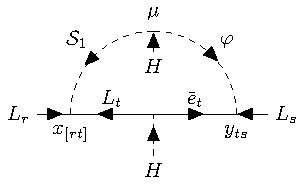
\includegraphics[width=0.45\textwidth]{zee_diag}
  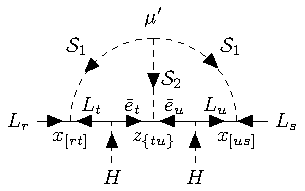
\includegraphics[width=0.45\textwidth]{zee_babu_diag}
  \caption{The neutrino self-energy diagrams relevant to the Zee (left) and
    Zee--Babu (right) models.}
  \label{fig:zee-and-zee-babu-diags}
\end{figure}

The Zee and Zee--Babu scenarios are only two of a very large number of radiative
models, none of which are \textit{a priori} more likely to be true than any
other. In the context of such a large theory-space, it is useful to have an
organising principle to aid in the study and classification of these models, and
beginning with $\Delta L = 2$ effective operators has been shown to be an
effective strategy.

One approach to this model taxonomy involves studying loop-level completions of
the Weinberg operator, and its dimension-($5+2n$) generalisations
\begin{equation*}
 \mathcal{O}_1^{\prime \cdots \prime} = (LL)HH(H^\dagger H)^n  \ .
\end{equation*}
Here, models can be systematically written down by studying the various
topologies able to be accommodated by the operator with increasing number of
loops. This is done in such a way that models implying lower-order contributions
to the neutrino mass can be discarded~\cite{Farzan:2012ev}. Such an approach has
been applied to the Weinberg operator up to three loops~\cite{Bonnet:2012kz,
  Sierra:2014rxa, Cepedello:2018rfh} and to its dimension-seven generalisation
at one loop~\cite{Cepedello:2017eqf}. An alternative and complementary method
begins by considering all of the gauge-invariant $\Delta L = 2$ operators in the
SM effective field theory (SMEFT), first listed in this context by Babu and
Leung~\cite{Babu:2001ex} and extended by de Gouv\^{e}a and
Jenkins~\cite{deGouvea:2007qla}. Supposing that the tree-level coefficient of
one of these is non-zero at the high scale, neutrino masses will be generated
from loop graphs contributing to the mixing of this operator and the
Weinberg-like operators $\mathcal{O}_1^{\prime \cdots \prime}$. The process of
expanding the operator into a series of UV-complete, renormalisable models that
generate the parent operator at tree-level is called \emph{opening up} or
\emph{exploding} the operator. The remaining external fields must be looped-off,
with additional loops of SM gauge bosons or Higgs fields added as necessary in
order to obtain a neutrino self-energy diagram. A model-building formula along
these lines has been formulated in Ref.~\cite{PhysRevD.87.073007}, and it has
been used to write down all of the minimal, tree-level UV-completions of
$\Delta L = 2$ operators at dimension seven~\cite{Cai:2014kra} corresponding to
tree-level and radiative neutrino-mass models. The tree-level completions of the
Weinberg-like operators have been written down up to dimension
eleven~\cite{Cai:2014kra, Bonnet:2009ej, Anamiati:2018cuq}. {\color{red}The
  $\Delta L = 2$ operators in the SM EFT are discussed in more detail in
  Sec.~\ref{sec:EFT-of-SM}.}

We note that an economic classification scheme, separate from an EFT framework,
was presented in Ref.~\cite{Klein:2019iws} based on the number of exotic degrees
of freedom by which the SM is extended. There, the method is applied to the case
of radiative models with two exotics\footnote{Including models with one scalar
  and one Dirac fermion.}, and has also been used to study minimal neutrino-mass
models compatible with $\mathrm{SU}(5)$ unification~\cite{Klein:2019jgb}.

\section{Effective field theory}

In the following we introduce EFT in general, and then specialise to those built
out of SM fields: the Standard Model EFT (SMEFT) and the Weak Effective Theory
(WET). We place particular emphasis on the operators appearing at dimension-six,
since these play an important role in phenomenological analyses. Much of the
focus of this work is the operators of odd mass-dimension up to dimension
eleven, which organise the building of neutrino-mass models in the tradition of
Refs.~\cite{Babu:2001ex, deGouvea:2007qla, PhysRevD.87.073007, Cai:2014kra}.
Many of the principles introduced here for the dimension-six SMEFT will be
directly relevant there. We begin with prefatory comments on the process of
tree-level matching, then move on to discuss the SMEFT and some of the
intricacies associated with redundancies among operators.

\subsection{Tree-level matching}
\label{sec:ch1-tree-level-matching}

Suppose one has a theory with light particle states described by fields
$\pi_{i}$ and heavy states described by $\Pi_{i}$ with a Lagrangian of the form
\begin{equation}
  \begin{aligned}
  \mathscr{L}_{\text{UV}}[\pi, \Pi] &= \mathscr{L}_{\text{kin}}[\pi, \Pi] + \mathscr{L}_{\text{int}}[\pi, \Pi], \text{ with } \\
  \mathscr{L}_{\text{int}}[\pi, \Pi] &= \mathscr{L}^{l}[\pi] + \mathscr{L}^{h}[\Pi] +  \mathscr{L}^{lh}[\pi, \Pi].
  \end{aligned}
\end{equation}
Below the threshold for $\Pi_{i}$ production, an effective description of the
theory can be used that involves interactions only between the light fields.
This effective theory is described by a Lagrangian
$\mathscr{L}_{\text{eff}}[\pi]$ involving interactions between the
$\pi_{i}$ that correspond to diagrams in the full theory containing only heavy
internal propagators and light external states. At the classical level,
$\mathscr{L}_{\text{eff}}$ can be written down by integrating out the
$\Pi_{i}$. Perturbatively this corresponds to expanding the heavy propagators
$\Delta$ in powers of momenta on the heavy mass scale\footnote{We note that some
  UV scenarios may have more than one characteristic scale. In this case
  $\Lambda$ can be understood as an effective scale which may not necessarily
  correspond to the mass of a specific particle.} $\Lambda$, such
that
\begin{equation}
  \label{eq:prop}
  \Delta = \begin{dcases}
    -\frac{1}{\Lambda^{2}}\left(1 + \frac{p^2}{\Lambda^{2}} + \cdots \right) & \text{for
    }\quad 
\includegraphics[width=0.17\linewidth]{scalar_prop.pdf} \\
    -\frac{\delta_{\alpha}^{\ \beta}}{\Lambda} \left( 1 + \frac{p^2}{\Lambda^{2}} + \cdots \right) & \text{for
    }\quad 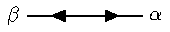
\includegraphics[width=0.17\linewidth]{fermion_mprop.pdf} \\
    -\frac{i p \cdot \bar{\sigma}^{\dot{\alpha}\beta}}{\Lambda^{2}} \left( 1 + \frac{p^2}{\Lambda^{2}} + \cdots \right) & \text{for
    }\quad 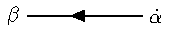
\includegraphics[width=0.17\linewidth]{fermion_pprop.pdf}
  \end{dcases}
  \ .
\end{equation}
In this notation, the arrow-preserving propagator corresponds to the part of the
regular four-component fermion propagator proportional to momentum, while the
arrow-violating one is the part proportional to the fermion mass. Expressions
for the fermion propagators with reversed arrows follow from
$\bar{\sigma}^{\mu} \to \sigma^{\mu}$ and interchanging dotted and undotted
indices (see Ref.~\cite{Dreiner:2008tw} Sec.~4.2 for the Lorentz structure).

Equivalently, the integration can be performed using the classical EOM of the
$\Pi_{i}$. For some heavy field $\Pi$, the linearised solution to its classical
EOM can be used to remove it from the Lagrangian completely. This procedure is
mildly different for scalars and fermions, and we briefly outline these
separately below. In both cases, we begin with a Lagrangian
$\mathscr{L}_{\text{UV}}$ for which we imagine that kinetic and mass mixing
terms between heavy and light fields have been removed.

There are tree-level contributions to $\mathscr{L}^{\text{eff}}$ as long as
there are interaction terms linear in $\Pi$. For scalar $\Pi$, the UV Lagrangian
contains the terms
\begin{equation}
  \label{eq:scalar-lag}
 \mathscr{L}_{\text{UV}}[\Pi, \pi] \supset \Pi^{\dagger} (- D^{2} - m_{\Pi}^{2}) \Pi + \left(\Pi \frac{\partial \mathscr{L}^{lh}}{\partial \Pi} + \text{h.c.} \right) \ ,
\end{equation}
where $\partial \mathscr{L}^{lh} / \partial \Pi$ is a function only of
light fields, and we are neglecting interactions of the form
$\Pi^{\dagger} \Pi f(\pi)$ for the sake of conciseness. The EOM are
\begin{equation}
  \label{eq:scalar-eom}
 (- D^{2} - m_{\Pi}^{2}) \Pi = - \frac{\partial \mathscr{L}^{lh}}{\partial \Pi^{\dagger}} + \mathcal{O}(\Pi^{2}) \ ,
\end{equation}
which can be solved for $\Pi^{\text{cl}}$, the classical field configuration, by
inverting the differential operator on the LHS of Eq.~\eqref{eq:scalar-eom} and
expanding in $D^{2} / m_{\Pi}^{2}$:
\begin{equation}
  \label{eq:scalar-repl}
  \Pi^{\text{cl}} = - \frac{1}{m_{\Pi}^{2}} \left( 1 - \frac{D^{2}}{m_{\Pi}^{2}}  + \cdots \right) \frac{\partial \mathscr{L}^{lh}}{\partial \Pi^{\dagger}} \ .
\end{equation}
This solution can be substituted back into Eq.~\eqref{eq:scalar-lag} to give
interactions between light fields in the tree-level effective Lagrangian:
\begin{equation}
  \label{eq:classical-efflag-scalar}
  \mathscr{L}_{\text{eff}}[\pi] \supset - \frac{\partial \mathscr{L}^{lh}}{\partial \Pi} \frac{1}{m_{\Pi}^{2}} \left( 1 - \frac{D^{2}}{m_{\Pi}^{2}} + \cdots \right) \frac{\partial \mathscr{L}^{lh}}{\partial \Pi^{\dagger}} \ .
\end{equation}
Many concrete examples of this procedure can be found in the literature, see
\textit{e.g.} Ref.~\cite{Henning:2014wua}. The expansion in $D^{2}/m_{\Pi}^{2}$
corresponds to the expansion in $p^{2} / \Lambda^{2}$ in the first case of
Eq.~\eqref{eq:prop}, showing the expansion of the scalar propagator.

Next we sketch out the procedure for a Dirac fermion
$\Pi + \bar{\Pi}^{\dagger}$, where $\Pi$ and $\bar{\Pi}$ are separate
two-component spin-$\tfrac{1}{2}$ fields transforming oppositely under
$G_{\text{SM}}$. In this case, the UV theory is described by a Lagrangian like
\begin{equation}
  \label{eq:fermion-lag}
  \mathscr{L}_{\text{UV}}[\Pi, \pi] \supset i \Pi^{\dagger} \bar{\sigma}^{\mu} D_{\mu} \Pi + i \bar{\Pi}^{\dagger} \bar{\sigma}^{\mu} D_{\mu} \bar{\Pi} + \left( \Pi \frac{\partial \mathscr{L}^{lh}}{\partial \Pi} + \bar{\Pi} \frac{\partial \mathscr{L}^{lh}}{\partial \bar{\Pi}} - m_{\Pi} \bar{\Pi} \Pi  + \text{h.c.} \right)
\end{equation}
Varying the action with respect to the heavy fields gives two coupled EOM:
\begin{align}
 i \bar{\sigma}^{\mu} D_{\mu} \Pi - m \bar{\Pi}^{\dagger} + \frac{\partial \mathscr{L}^{lh}}{\partial \Pi^{\dagger}} &= 0 \ , \label{eq:pi-fermion-eom} \\
 i \bar{\sigma}^{\mu} D_{\mu} \bar{\Pi} - m \Pi^{\dagger} + \frac{\partial \mathscr{L}^{lh}}{\partial \bar{\Pi}^{\dagger}} &= 0 \ . \label{eq:pibar-fermion-eom}
\end{align}
Substituting Eq.~\eqref{eq:pi-fermion-eom} into Eq.~\eqref{eq:pibar-fermion-eom}
gives a second-order partial differential equation in $\Pi$, analogous to
Eq.~\eqref{eq:scalar-eom}. Inverting the differential operator in a similar way
gives
\begin{equation}
  \label{eq:fermion-repl}
  \Pi^{\text{cl}}_{\beta} = \frac{1}{m_{\Pi}^{2}} \left( \epsilon_{\alpha \beta} + \frac{ \tfrac{1}{2} X_{\alpha \beta} - D^{2} \epsilon_{\alpha \beta}}{m_{\Pi}^{2}} + \cdots \right) \left( i D^{\alpha \dot{\alpha}} \frac{\partial \mathscr{L}^{lh}}{\partial \Pi^{\dagger}_{\dot{\beta}}} \epsilon_{\dot{\alpha} \dot{\beta}} + m_{\Pi} \frac{\partial \mathscr{L}^{lh}}{\partial \bar{\Pi}_{\alpha}} \right) \ ,
\end{equation}
where the field-strength tensor comes about from a structure like
\begin{align}
  [\sigma^{\mu} \bar{\sigma}^{\nu}]_{\alpha}^{\ \beta} D_{\mu} D_{\nu} &= \eta^{\mu\nu} D_{\mu} D_{\nu} \delta_{\alpha}^{\ \beta} - 2i [\sigma^{\mu\nu}]_{\alpha}^{\ \beta} D_{\mu} D_{\nu} \\
  &= D^{2} \delta_{\alpha}^{\ \beta} - \tfrac{1}{2} X_{\alpha}^{\ \beta} \ .
\end{align}
Here, and later in this section, the replacement $\bar{\Pi} \to \Pi$ should be
understood for Majorana $\Pi$. Each contribution corresponds to a particular
kind of propagator in the perturbative picture. The first term in the last
parenthesis of Eq.~\eqref{eq:fermion-repl} results from the fermion propagator
proportional to momentum: the arrow-preserving fermion propagator shown as the
last case of Eq.~\eqref{eq:prop}. The second term in the same parentheses stems
from the fermion propagator proportional to the mass, corresponding to the
arrow-violating propagator shown in the middle case of Eq.~\eqref{eq:prop}.
Replacing $\Pi$ in Eq.~\eqref{eq:fermion-lag} gives the tree-level effective
Lagrangian with the heavy fermion integrated out:
\begin{equation}
  \begin{aligned}
  \label{eq:classical-efflag-fermion}
  \mathscr{L}_{\text{eff}}[\pi] &\supset \frac{\partial \mathscr{L}^{lh}}{\partial \Pi_{\beta}} \frac{1}{m_{\Pi}^{2}} \left(\epsilon_{\alpha \beta} + \frac{ \tfrac{1}{2} X_{\alpha \beta} - D^{2} \epsilon_{\alpha \beta}}{m_{\Pi}^{2}} +  \cdots \right) i D^{\alpha \dot{\alpha}} \frac{\partial \mathscr{L}^{lh}}{\partial \Pi^{\dagger}_{\dot{\beta}}} \epsilon_{\dot{\alpha} \dot{\beta}}\\
  &\quad + \frac{\partial \mathscr{L}^{lh}}{\partial \Pi_{\beta}} \frac{1}{m_{\Pi}^{2}} \left(\epsilon_{\alpha \beta} + \frac{ \tfrac{1}{2} X_{\alpha \beta} - D^{2} \epsilon_{\alpha \beta}}{m_{\Pi}^{2}} + \cdots \right) \frac{\partial \mathscr{L}^{lh}}{\partial \bar{\Pi}_{\alpha}} \ .
  \end{aligned}
\end{equation}

As shown in Eqs.~\eqref{eq:classical-efflag-scalar} and
\eqref{eq:classical-efflag-fermion}, expanding in powers of derivatives on heavy
masses leads to a tower of local operators of increasing mass dimension $d_{i}$
organised as a power series in the inverse heavy scale:
\begin{equation}
  \mathscr{L}_{\text{eff}}[\pi] = \mathscr{L}^{l}[\pi] + \sum_{i} \frac{C_{i}}{\Lambda^{d_{i}-4}} \mathcal{O}_{i}[\pi].
\end{equation}
The $C_{i}$ are dimensionless coefficients which are in general calculable if
one knows the high-energy theory.

\subsection{Effective field theories of the SM}
\label{sec:EFT-of-SM}

Below we discuss EFTs constructed from SM fields and invariant under SM
symmetries. The main theory of study is the SMEFT: the gauge- and
Lorentz-invariant EFT built from the fields listed in Table~\ref{tab:sm-fields}.
We also mention the WET, also known as the LEFT (Low-energy Effective Field
Theory), for which invariance under
$\mathrm{SU}(2)_{+} \otimes \mathrm{SU}(2)_{-} \otimes \mathrm{SU}(3)_{c} \otimes \mathrm{U}(1)_{\text{EM}}$
is required.

\subsubsection{The SMEFT at dimension six}

Given the broad experimental success of the SM, it is perhaps a sensible
assumption that there should be a sizeable mass gap between the electroweak
scale and the mass-scale characterising any new physics. In this context, the
SMEFT can be a powerful tool for constraining how this new physics might look in
a model-independent way. Indeed, the SMEFT operators at dimension six are
already coming to play an increasingly important role in particle phenomenology,
and they have become the \textit{de facto} framework for interpreting low-energy
constraints on theoretical models and experimental deviations from SM
predictions. For an extensive review, we point the reader to
Ref.~\cite{Brivio:2017vri}.

It has not been easy to write down a complete basis of operators in the
SMEFT~\cite{Buchmuller:1985jz, Grzadkowski:2010es}, although this is now a
mostly solved problem~\cite{Lehman:2015via, Henning:2015daa, Lehman:2015coa,
  Henning:2015alf, Henning:2017fpj}. The lowest-dimensional operator appearing
in the EFT is also the only dimension-five operator:
\begin{equation}
  \mathscr{L}^{(5)} = [C_{5}]_{\{rs\}} (L^{i}_{r} L^{j}_{s}) H^{k} H^{l} \epsilon_{ik} \epsilon_{jl} + \text{h.c.} \ ,
\end{equation}
already discussed briefly in Sec.~\ref{sec:models-of-mv}. The matrix of operator
coefficients is necessarily symmetric by Fermi--Dirac statistics. The operator
violates lepton-number by two units, and usually gives the dominant contribution
to the neutrino mass in Majorana models. Ref.~\cite{Kobach:2016ami} shows that
operators in the SMEFT of mass-dimension $d$ satisfy
\begin{equation}
  \frac{1}{2} (\Delta B - \Delta L) = d \mod 2 \ ,
\end{equation}
and thus odd mass-dimension operators must violate $B - L$ by two units, while
operators of even mass-dimension cannot violate $B - L$. So, aside from
lepton-number-violating effects, the leading-order deviations from the SM appear
at dimension six, where there are many more operators.

The dimension-six operators come in eight general classes: $X^{3}$, $H^{6}$,
$H^{4}D^{2}$, $X^{2}H^{2}$, $\psi^{2}H^{3}$, $\psi^{2}XH$, $\psi^{2}H^{2}D$ and
$\psi^{4}$. (Here, $X$ represents a general field-strength tensor, $D$ is a
covariant derivative and $\psi$ is a fermion field.) The $\psi^{4}$-type
operators illustrate some of the difficulties encountered when writing down a
complete basis of operators, since they can be simplified by Fierz and Schouten
identities relating to the spinor, isospin and colour structure. The most common
basis found in the literature is the Warsaw basis~\cite{Buchmuller:1985jz,
  Grzadkowski:2010es}, which tends to prefer vector currents for fermions. Thus,
for example, the four-fermion operators with field content $L^{4}$ written in
this way are
\begin{align}
  [\mathcal{O}_{ll}]_{rstu} &= (L^{\dagger}_r \bar{\sigma}_{\mu} L_s) (L^{\dagger}_t \bar{\sigma}_{\mu} L_u) \ , \\
  [\mathcal{O}_{ll}^{(3)}]_{rstu} &= (L_r^{\dagger} \bar{\sigma}_{\mu} \tau^I L_s) (L_t^{\dagger} \bar{\sigma}_{\mu} \tau^I L_u) \ .
\end{align}
Here $\mathcal{O}_{ll}^{(3)}$ contracts the
$\bar{\mathbf{2}} \otimes \mathbf{2}$ of the $L^{\dagger}$ and $L$ into the
triplet representation. Naively there seem to be two operators, however
$\mathcal{O}_{ll}^{(3)}$ can be rewritten using the $\mathrm{SU}(2)$ Fierz
identity
\begin{equation}
  [\tau^{I}]^{i}_{\ j} [\tau^{I}]^{k}_{\ l} = 2\delta^{i}_{\ m} \delta^{k}_{\ j} - \delta^{i}_{\ j} \delta^{k}_{\ l}
\end{equation}
and the related identity acting on the spinor structure
\begin{equation}
  \label{eq:spinor-fierz}
  (\psi_{1}^{\dagger} \bar{\sigma}^{\mu} \psi_{2})  (\psi_{3}^{\dagger} \bar{\sigma}^{\mu} \psi_{4}) = (\psi_{1}^{\dagger} \bar{\sigma}^{\mu} \psi_{4})  (\psi_{3}^{\dagger} \bar{\sigma}^{\mu} \psi_{2})
\end{equation}
such that
\begin{equation}
  [\mathcal{O}_{ll}^{(3)}]_{rstu} = 2 [\mathcal{O}_{ll}]_{ruts} - [\mathcal{O}_{ll}]_{rstu} \ .
\end{equation}
Thus, the operators $[\mathcal{O}_{ll}^{(3)}]_{rstu}$ can be expressed as linear
combinations of the $[\mathcal{O}_{ll}]_{rstu}$, and both operators should not
be included in a genuine basis. The situation is slightly more complicated for
the four-quark operators, since there is an additional space of indices to
handle. In the case of operators with field content $Q^{4}$, there seem to
naively be four invariants, which can be written as vector currents
\begin{equation}
  (Q^{\dagger} \bar{\sigma}_{\mu} \Gamma Q) (Q^{\dagger} \bar{\sigma}_{\mu} \Gamma Q) \ ,
\end{equation}
where the possible structures $\Gamma \otimes \Gamma$ can be expressed schematically as
\begin{equation}
  1 \otimes 1,\quad \tau^{I} \otimes \tau^{I},\quad \lambda^{A} \otimes \lambda^{A},\quad \tau^{I} \lambda^{A} \otimes \tau^{I} \lambda^{A} \ .
\end{equation}
The $\mathrm{SU}(2)_{L}$ and $\mathrm{SU}(3)_{c}$ index contraction can either
be internal to the fermion current, or it may connect fermions in adjacent
currents. For example, the $\mathrm{SU}(2)_{L}$ contraction is internal for the
structures $1 \otimes 1$ and $\lambda^{A} \otimes \lambda^{A}$, but external for
$\tau^{I} \otimes \tau^{I}$ and
$\tau^{I} \lambda^{A} \otimes \tau^{I} \lambda^{A}$. The spinor identity
Eq.~\eqref{eq:spinor-fierz} exchanges the $Q$ fields, so it interchanges the
isospin and colour indices so that
\begin{equation}
  \text{both internal} \leftrightarrow \text{both external},\quad \mathrm{SU}(2)_{L} \text{ external} \leftrightarrow \mathrm{SU}(3)_{c} \text{ external} \ .
\end{equation}
This means only two of the four invariants are independent. These are chosen to
be $1 \otimes 1$ and $\tau^{I} \otimes \tau^{I}$ in the Warsaw basis.

The operators in the Warsaw basis are listed in Tables~\ref{tab:smeft-d6-psi4}
and \ref{tab:smeft-d6-other}. This is the form in which we use the operators
throughout the rest of this work. Each operator is given in four-component
spinor notation, as is usual in the literature. We refer the reader to
Appendix~\ref{chapter:notation} for the correspondence to the two-component
notation we use elsewhere, along with other relevant mathematical notation used
in the tables. Our conventions are chosen to comply with those of
Ref.~\cite{Aebischer:2017ugx}.

\begin{table}
  \begin{center}
    \begin{tabular}{cclccl}
      \toprule
      & Operator & Label & & Operator & Label \\
      \cmidrule{2-3} \cmidrule{5-6}
      %
      % 4F: LLLL
      \multirow{3}{*}
      {$(\bar{L} L ) (\bar{L} L )$} & $(\bar{L} \gamma_\mu L) (\bar{L} \gamma^\mu L)$ & $\mathcal{O}_{ll}$ &
      & & \\
      %
      &
      $(\bar{Q} \gamma_\mu Q) (\bar{Q} \gamma^\mu Q)$ & $\mathcal{O}_{qq}^{(1)}$ &
      &
      $(\bar{Q} \gamma_\mu \tau^{I} Q )
      (\bar{Q} \gamma^\mu \sigma^I Q)$ &
      $\mathcal{O}_{qq}^{(3)}$ \\
      %
      &
      $(\bar{L} \gamma_\mu L )
      (\bar{Q} \gamma^\mu Q )$ &
      $\mathcal{O}_{lq}^{(1)}$ &
      &
      $(\bar{L} \gamma_\mu\sigma^I L)
      (\bar{Q} \gamma^\mu \sigma^I Q)$ &
      $\mathcal{O}_{lq}^{(3)}$ \\[1mm]
      %
      \midrule[0.25mm]
      % 4F: RRRR
      \multirow{4}{*}
      {$(\bar{R}R)(\bar{R}R)$} &
      $(\bar{e}_R \gamma_\mu e_R)
      (\bar{e}_R \gamma^\mu e_R)$ &
      $\mathcal{O}_{ee}$ &
      & \\
      %
      &
      $(\bar{u}_R \gamma_\mu u_R)
      (\bar{u}_R \gamma^\mu u_R)$ &
      $\mathcal{O}_{uu}$ &
      &
      $(\bar{d}_R \gamma_\mu d_R)
      (\bar{d}_R \gamma^\mu d_R)$ &
      $\mathcal{O}_{dd}$ \\
      %
      &
      $(\bar{u}_R \gamma_\mu u_R)
      (\bar{d}_R \gamma^\mu d_R)$ &
      $\mathcal{O}_{ud}^{(1)}$ &
      &
      $(\bar{u}_R \gamma_\mu \lambda^A u_R)
      (\bar{d}_R \gamma^\mu \lambda^A d_R)$ &
      $\mathcal{O}_{ud}^{(8)}$ \\
      %
      &
      $(\bar{e}_R \gamma_\mu e_R)
      (\bar{u}_R \gamma^\mu u_R)$ &
      $\mathcal{O}_{eu}$ &
      &
      $(\bar{e}_R \gamma_\mu e_R)
      (\bar{d}_R \gamma^\mu d_R)$ &
      $\mathcal{O}_{ed}$ \\[1mm]
      %
      \midrule[0.25mm]
      % 4F: LLRR
      \multirow{4}{*}
      {$(\bar{L}L)(\bar{R}R)$} &
      $(\bar{L} \gamma_\mu L)
      (\bar{e}_R \gamma^\mu e_R)$ &
      $\mathcal{O}_{le}$ &
      &
      $(\bar{Q} \gamma_\mu Q)
      (\bar{e}_R \gamma^\mu e_R)$
      &
      $\mathcal{O}_{qe}$ \\
      %
      &
      $(\bar{L} \gamma_\mu L)
      (\bar{u}_R \gamma^\mu u_R)$ &
      $\mathcal{O}_{lu}$ &
      &
      $(\bar{L} \gamma_\mu L)
      (\bar{d}_R \gamma^\mu d_R)$ &
      $\mathcal{O}_{ld}$ \\
      %
      &
      $(\bar{Q} \gamma_\mu Q)
      (\bar{u}_R \gamma^\mu u_R)$ &
      $\mathcal{O}_{qu}^{(1)}$ &
      &
      $(\bar{Q} \gamma_\mu \lambda^A Q_L)
      (\bar{u}_R \gamma^\mu \lambda^A u_R)$ &
      $\mathcal{O}_{qu}^{(8)}$ \\
      %
      &
      $(\bar{Q} \gamma_\mu Q)
      (\bar{d}_R \gamma^\mu d_R)$ &
      $\mathcal{O}_{qd}^{(1)}$ &
      &
      $(\bar{Q} \gamma_\mu \lambda^{A} Q_L)
      (\bar{d}_R \gamma^\mu \lambda^{A} d_R)$ &
      $\mathcal{O}_{qd}^{(8)}$ \\[1mm]
      %
      \midrule[0.25mm]
      % 4F:LRRL &  LRLR
      $(\bar{L}R)(\bar{R}L)$ &
      $(\bar{L} e_R) (\bar{d}_R Q)$ &
      $\mathcal{O}_{ledq}$ &
      & & \\[1mm]
      \midrule[0.25mm]
      \multirow{2}{*}
      {$(\bar{L}R)(\bar{L}R)$} &
      $(\bar{Q}_{i}  u_R) (\bar{Q}_{j} d_R) \epsilon^{ij}$ &
      $\mathcal{O}_{quqd}^{(1)}$ &
      &
      $(\bar{Q}_{i} \lambda^{A} u_R) (\bar{Q}_{j} \lambda^{A} d_R) \epsilon^{ij}$ &
      $\mathcal{O}_{quqd}^{(8)}$ \\
      %
      &
      $(\bar{L}_{i}  e_R) (\bar{Q}_{j} u_R) \epsilon^{ij}$ &
      $\mathcal{O}^{(1)}_{lequ}$ &
      &
      $(\bar{L}_{i}  \sigma_{\mu\nu} e_R) (\bar{Q}_{j} \sigma^{\mu\nu} u_R) \epsilon^{ij}$ &
      $\mathcal{O}^{(3)}_{lequ}$ \\[1mm]
      %
      \midrule[0.25mm]
      %
      \multirow{4}{*}
      {$\Delta B = 1$} &
      \multicolumn{4}{r}{
        $(d^{a}_R u^b_R) (Q^{ci} L^{j})\epsilon_{abc} \epsilon_{ij}$} &
      $\mathcal{O}_{duq}$ \\
      &
      \multicolumn{4}{r}{
        $(Q^{ai} Q^{bj})
        (u^{c}_R e_R) \epsilon_{abc} \epsilon_{ij}$} &
      $\mathcal{O}_{qqu}$ \\
      &
      \multicolumn{4}{r}{
        $(d^{a}_R u^b_R) (u^{c}_R e_R) \epsilon_{abc}$} &
      $\mathcal{O}_{duu}$ \\
      &
      \multicolumn{4}{r}{
        $ (Q^{ai} Q^{bk}) (Q^{cl} L^{j}) \epsilon_{abc} \epsilon_{ij} \epsilon_{kl}$} &
      $\mathcal{O}_{qqq}$ \\[1mm]
      \bottomrule
    \end{tabular}
    \caption{The table shows the four-fermion operators in the dimension-six
      SMEFT in the Warsaw basis~\cite{Buchmuller:1985jz, Grzadkowski:2010es}.
      The operators are listed in four-component spinor notation, and a full
      correspondence to the two-component notation we use elsewhere can be found
      in Appendix~\ref{chapter:notation}. We remind the reader that
      combinations like $(Q Q)$ stand for $(\bar{Q}^{C} Q)$, where $Q^{C}$ is
      the charge-conjugated spinor. Flavor indices are omitted, and should be
      understood to label the fermions in the order $\{r, s, t, u\}$ as they
      appear. \label{tab:smeft-d6-psi4}}
  \end{center}
\end{table}

\begin{table}
  \begin{center}
    \begin{tabular}{cclccl}
      \toprule
      & Operator & Notation & & Operator & Notation \\
      \cmidrule{2-3} \cmidrule{5-6}
      % X^3
      \multirow{2}{*}{$X^3$}
      &
      $W^{I\nu }_{\mu} W^{J\rho}_{\nu} W^{K \mu}_{\rho} \epsilon_{IJK} $ &
      $\mathcal{O}_{W}$ &
      &
      $\tilde{W}^{I \nu}_{\mu} W^{J\rho}_{\nu} W^{K\mu}_{\rho} \epsilon_{IJK}$ &
      $\mathcal{O}_{\tilde{W}}$ \\
      %
      &
      $G^{A\nu}_\mu G^{B\rho}_\nu G^{C\mu}_\rho f_{ABC}$ &
      $\mathcal{O}_{G}$ &
      &
      $\tilde{G}^{A\nu}_\mu G^{B\rho}_\nu G^{C\mu}_\rho f_{ABC}$ &
      $\mathcal{O}_{\tilde{G}}$ \\[1mm]
      \midrule[0.25mm]
      \vspace{-5mm} & & & & \\
      % phi^6
      $H^6$ &
      $(H^{\dagger} H)^3$ &
      $\mathcal{O}_{H}$ &
      & & \\[1mm]
      \midrule[0.25mm]
      \vspace{-5mm} & & & & \\
      % phi^4 D^2
      $H^4 D^2$ &
      $(H^{\dagger} H )\Box (H^{\dagger} H)$ &
      $\mathcal{O}_{H \Box}$ &
      &
      $H^{\dagger}_{i} (D_\mu H)^{i} \cdot (D^\mu H)_{j}^{\dagger} H^{j}$ &
      $\mathcal{O}_{H D}$ \\[1mm]
      %
      \midrule[0.25mm]
      % psi^2 phi^3
      \multirow{2}{*}{$\psi^2 H^2$} &
      $(H^{\dagger} H) (\bar{L} H e_R)$ &
      $\mathcal{O}_{e H}$ & & \\
      &
      $(H^{\dagger} H)
      (\bar{Q} H d_R)$ &
      $\mathcal{O}_{d H}$ &
      &
      $(H^{\dagger} H)
      (\bar{Q} \tilde{H} u_R )$ &
      $\mathcal{O}_{u H}$ \\[1mm]
      \midrule[0.25mm]
       % X^2 \phi^2
      \multirow{4}{*}{$X^2 H^2$} &
      $(H^\dagger H) B_{\mu\nu} B^{\mu\nu} $ &
      $\mathcal{O}_{H B}$ &
      &
      $(H^\dagger H) \tilde{B}_{\mu\nu} B^{\mu\nu}$ &
      $\mathcal{O}_{H \tilde{B}}$ \\
      %
      &
      $(H^\dagger H) W_{\mu\nu}^I W^{I\mu\nu} $ &
      $\mathcal{O}_{H W}$ &
      &
      $(H^\dagger H) \tilde{W}_{\mu\nu}^I W^{I\mu\nu}$ &
      $\mathcal{O}_{H \tilde{W}}$ \\
      %
      &
      $(H^\dagger \tau^I H) W^I_{\mu\nu} B^{\mu\nu}$ &
      $\mathcal{O}_{H WB}$ &
      &
      $(H^\dagger \tau^I H) \tilde{W}^I_{\mu\nu} B^{\mu\nu}$ &
      $\mathcal{O}_{H\tilde{W}B}$ \\
      %
      &
      $(H^\dagger H) G_{\mu\nu}^A G^{A\mu\nu} $ &
      $\mathcal{O}_{H G}$ &
      &
      $(H^\dagger H) \tilde{G}_{\mu\nu}^A G^{A\mu\nu}$ &
      $\mathcal{O}_{H\tilde{G}}$ \\[1mm]
      %
      \midrule[0.25mm]
      % psi^2 X phi
      \multirow{4}{*}{$\psi^2 X H$} &
      $(\bar{L} \sigma^{\mu\nu} e_R)
      H B_{\mu\nu}$ &
      $\mathcal{O}_{eB}$ &
      &
      $(\bar{L} \sigma^{\mu\nu} e_R)
      \tau^I H W_{\mu\nu}^I$ &
      $\mathcal{O}_{eW}$ \\
      %
      & $(\bar{Q} \sigma^{\mu\nu} u_R)
      \tilde{H} B_{\mu\nu}$ &
      $\mathcal{O}_{uB}$ &
      &
      $(\bar{Q} \sigma^{\mu\nu} u_R)
      \tau^I \tilde{H} W_{\mu\nu}^I$ &
      $\mathcal{O}_{uW}$ \\
      %
      &
      $(\bar{Q} \sigma^{\mu\nu} d_R) H B_{\mu\nu}$ &
      $\mathcal{O}_{dB}$ &
      &
      $(\bar{Q} \sigma^{\mu\nu} d_R)
      \tau^I H W_{\mu\nu}^I$ &
      $\mathcal{O}_{dW}$ \\
      %
      &
      $(\bar{Q} \sigma^{\mu\nu} \lambda^A u_R )
      \tilde{H} G_{\mu\nu}^A$ &
      $\mathcal{O}_{uG}$ &
      &
      $(\bar{Q} \sigma^{\mu\nu} \lambda^{A} d_R) H G^A_{\mu\nu}$ &
      $\mathcal{O}_{dG}$ \\[1mm]
      %
      \midrule[0.25mm]
      % psi^2 phi^2 D
      \multirow{5}{*}{$\psi^2 H^2 D$} &
      $(H^{\dagger} i\bar{D}_\mu H)
      (\bar{L} \gamma^\mu L )$ &
      $\mathcal{O}_{H l}^{(1)}$ &
      &
      $(H^{\dagger} i\bar{D}^{I}_\mu H)
      (\bar{L} \gamma^\mu \tau^{I} L )$ &
      $\mathcal{O}_{H l}^{(3)}$ \\
      %
      &
      $(H^{\dagger} i\bar{D}_\mu H)
      (\bar{e}_R \gamma^\mu e_R)$ &
      $\mathcal{O}_{H e}$ &
      & & \\
      %
      &
      $(H^{\dagger} i\bar{D}_\mu H)
      (\bar{Q} \gamma^\mu Q)$ &
      $\mathcal{O}_{H q}^{(1)}$ &
      &
      $(H^{\dagger} i\bar{D}^{I}_\mu H)
      (\bar{Q} \gamma^\mu \tau^{I} Q )$ &
      $\mathcal{O}_{H q}^{(3)}$ \\
      %
      &
      $(H^{\dagger} i\bar{D}_\mu H)
      (\bar{u}_R \gamma^\mu u_R)$ &
      $\mathcal{O}_{H u}$ &
      &
      $(H^{\dagger} i\bar{D}_\mu H)
      (\bar{d}_R \gamma^\mu d_R)$ &
      $\mathcal{O}_{H d}$ \\
      %
      &
      $H^{i} (iD_\mu H)^{j} \epsilon_{ij} \cdot
      (\bar{u}_R \gamma^\mu d_R)$ &
      $\mathcal{O}_{H ud}$ &
      & & \\[1mm]
      \bottomrule
    \end{tabular}
    \caption{The table shows the operators featuring in the Warsaw
      basis~\cite{Buchmuller:1985jz, Grzadkowski:2010es} of the dimension-six
      SMEFT that are not four-fermion operators. We point the reader to
      Appendix~\ref{chapter:notation} for the correspondence between the
      four-component notation used here and the two-component notation used
      elsewhere in this work for spinors, along with the definition of
      $\bar{D}^{\mu}$. Flavor indices are omitted and should be understood to
      act on fermions in the order $\{r, s\}$ as they appear in each
      operator. \label{tab:smeft-d6-other}}
  \end{center}
\end{table}

\subsubsection{The Low-energy or Weak Effective Theory}

Many experimental constraints on the SM and its extensions come from low-energy
flavour-changing process involving four fermions. These can be accurately
described using an effective theory, similar to the Fermi theory of the Weak
interactions, in which the electroweak gauge bosons, the physical higgs and the
top quark have been integrated out. The dimension six operators in this
low-energy EFT~\cite{Jenkins:2017jig, Aebischer:2017gaw, Jenkins:2017dyc,
  Aebischer:2015fzz} have been extensively applied to $B$, $K$ and $D$ meson
decays, meson--anti-meson oscillations and leptonic decays,
\textit{e.g.}~\cite{Buchalla:1995vs}. They are also an invaluable tool for
studying deviations from the SM in a way independent from many of the
assumptions underlying SMEFT. The symmetries of the theory are only those of QCD
and electromagnetism, and the fermions are the usual quarks and leptons with the
top quark excluded from the theory. At dimension six there are 3,631
$\Delta B = \Delta L = 0$ operators~\cite{Jenkins:2017jig}, and we do not list
them all here. Rather, we introduce the pertinent operators within the
discussion of each specific phenomenological process we study in this work.

\subsection{Operator redundancy and the Hilbert series}

The previous section introduced some of the difficulties involved with writing
down a basis of four-fermion operators for a complex EFT like the SMEFT.
Additional redundancy can occur once operators with (covariant) derivatives are
included. These include operator relations through integration by parts (IBP)
and field redefinitions involving the classical equations of motion
(EOM)~\cite{Buchmuller:1985jz, Arzt:1993gz, Georgi:1991ch}. At mass-dimensions
larger than six, these come to be a large source of the difficulty in writing
down a complete operator basis, but the problem can be addressed through
Hilbert-series methods~\cite{Lehman:2015via, Henning:2015daa, Lehman:2015coa,
  Henning:2015alf, Henning:2017fpj}. Below, we motivate how the EOM can be used
to simplify effective operator bases, and explain how these redundancies can be
accounted for through Hilbert series techniques.

\subsubsection{Field redefinitions and the equations of motion}
\label{sec:eom}

It is clear that operators can be simplified using the EOM at lowest
order~\cite{Buchmuller:1985jz, Gasser:1983yg, Gasser:1984gg, DeRujula:1991ufe},
since the external legs are put on-shell in the Feynman rules. That is, an
operator like
\begin{equation}
  (H^{\dagger} H) (\bar{e}_{R} i \slashed{D} e_{R})
\end{equation}
can be simplified when it appears in calculations with all legs external. So,
any leading-order amplitude involving the operator can be reduced through
\begin{equation}
  i \slashed{D} e_{R} = y_{e} H^{\dagger} L \ ,
\end{equation}
(or equivalently $\mathcal{M} \sim \slashed{p} u_{e} = m_{e} u_{e}$ by the
momentum-space Dirac equation) to $\mathcal{O}_{eH}$. Surprisingly, this useful
result can be extended even to cases involving propagators and loops by
performing field redefinitions. Specifically, field redefinitions that preserve
the symmetries of the theory and contain a term linear in the original field
allow the EOM to simplify a local effective Lagrangian without affecting the
$S$-matrix~\cite{CHISHOLM1961469, Kamefuchi:1961sb, divakaran1963equivalence, Bergere:1975tr, SHARATCHANDRA1978408, PhysRevD.2.2869, Kallosh:1972ap}. We illustrate this with a
toy $\phi^{4}$ theory:
\begin{equation}
  \label{eq:toy-phi4}
  \mathscr{L} = \frac{1}{2}(\partial_{\mu} \phi) (\partial^{\mu} \phi) - \frac{1}{2} m^{2} \phi^{2} - \frac{\lambda}{4!} \phi^{4} + \frac{c_{1}}{\Lambda^{2}} \phi^{6} + \frac{c_{2}}{\Lambda^{2}} \phi^{3} \Box \phi + \mathcal{O}(\Lambda^{-4}) \ .
\end{equation}
Under the field redefinition
\begin{equation}
  \label{eq:phi-redef}
  \phi \to \phi + \frac{c_{2}}{\Lambda^{2}} \phi^{3} \ ,
\end{equation}
the kinetic term becomes
\begin{equation}
  \frac{1}{2}(\partial_{\mu} \phi) (\partial^{\mu} \phi) \to  \frac{1}{2}(\partial_{\mu} \phi) (\partial^{\mu} \phi) - \frac{c_{2}}{\Lambda^{2}} \phi^{3} \Box \phi + \mathcal{O}(\Lambda^{-4}) \ ,
\end{equation}
where the second term comes from integrating
$c_{2} \Lambda^{-2} (\partial_{\mu} \phi) (\partial^{\mu} \phi^{3})$ by parts.
This term cancels the last term in Eq.~\eqref{eq:toy-phi4}, for which the
additional operators induced by the field redefinition are all
$\mathcal{O}(\Lambda^{-4})$ terms. Performing the field redefinition on the
other interaction terms in the Lagrangian leads to an effective redefinition of
$\lambda$ and $c_{1}$, with all other induced operators suppressed by four
powers of $\Lambda$. Concretely,
\begin{equation}
  \begin{aligned}
    \mathscr{L} &\to \frac{1}{2} (\partial_{\mu} \phi) (\partial^{\mu} \phi) - \frac{1}{2} m^{2} \phi^{2} - \frac{\lambda}{4!} \phi^{4} + \frac{c_{1}}{\Lambda^{2}} \phi^{6} + \frac{c_{2}}{\Lambda^{2}} \phi^{3} \Box \phi \\
    &\quad + \frac{c_{2}}{\Lambda^{2}} \phi^{3} \underbracket{\left( - \Box \phi - m^{2} \phi - \frac{\lambda}{3!}\phi^{3} \right)}_{\equiv E[\phi]} + \cdots \\
    &= \frac{1}{2} (\partial_{\mu} \phi) (\partial^{\mu} \phi) - \frac{1}{2} m^{2} \phi^{2} - \underbracket{\left( \frac{\lambda}{4!} + \frac{c_{2}}{\Lambda^{2}}m^{2} \right)}_{\equiv \lambda^{\prime} / 4!} \phi^{4} + \underbracket{\left( \frac{c_{1}}{\Lambda^{2}} - \frac{c_{2}}{\Lambda^{2}} \frac{\lambda}{3!} \right)}_{\equiv c^{\prime}_{1} / \Lambda^{2}}\phi^{6} + \mathcal{O}(\Lambda^{-4}) \ .
  \end{aligned}
\end{equation}
This is guaranteed since in the effective theory all of the operators consistent
with the symmetries are already present, so the effects of the additional terms
are exclusively to shift the coefficients of the theory around. The appearance
of the EOM operator $E[\phi]$ above can be understood on the basis of the nature
of the field redefinition Eq.~\eqref{eq:phi-redef}. The additional terms induced
by the field redefinition up to $\mathcal{O}(\Lambda^{-2})$ will be those in
which a $\phi$ or its derivative has been replaced with
$c_{2} \Lambda^{-2} \phi^{3}$. That is,
\begin{equation}
  \begin{aligned}
    \Delta \mathscr{L} &= \frac{c_{2}}{\Lambda^{2}} \phi^{3} \frac{\partial \mathscr{L}}{\partial \phi} + \frac{c_{2}}{\Lambda^{2}} (\partial_{\mu} \phi^{3}) \frac{\partial \mathscr{L}}{\partial (\partial_{\mu} \phi)} + \mathcal{O}(\Lambda^{-4}) \\
    &= \frac{c_{2}}{\Lambda^{2}} \phi^{3} \left[ \frac{\partial \mathscr{L}}{\partial \phi} - \partial_{\mu} \frac{\partial \mathscr{L}}{\partial (\partial_{\mu} \phi)} \right]  + \mathcal{O}(\Lambda^{-4}) \ ,
  \end{aligned}
\end{equation}
where we have integrated the second term by parts in the last step. In order to
show that the $S$-matrix is unaffected, it is not sufficient to show only that
the Lagrangian has not changed form (up to order $\Lambda^{-2}$). In the path
integral picture, the field redefinition Eq.~\eqref{eq:phi-redef} will also
change the measure of the path integral and the sources $\mathcal{J}_{i}$ for
each of the fields, whose effects we have not considered. These additional
changes can be dealt with generically~\cite{Arzt:1993gz}. In short, the Jacobian
can be written as a Lagrangian involving ghost fields, similar to the
Fadeev--Popov approach taken in Gauge Theory. In this case the ghost fields
acquire a mass of order $\Lambda$, and are therefore not relevant to the
effective theory. The change to the source $\mathcal{J}_{\phi}$ does lead to a
change in the Green's functions of the theory, although the $S$-matrix remains
unchanged. We can see this easily in our toy theory. The LSZ reduction
formula~\cite{Lehmann:1954rq}
\begin{equation}
  \begin{aligned}
    &G^{(n+m)}(q_{1}, \ldots, q_{m}; p_{1}, \ldots, p_{n}) \\
    &\quad \underset{\substack{p_{j}^{2} \to m^{2}\\q_{k}^{2} \to m^{2}}}{\sim} \left(\prod_{j=1}^{m} \frac{i \sqrt{Z_{j}}}{p_{j}^{2} - m^{2} + i\epsilon}\right) \left(\prod_{k=1}^{n} \frac{i \sqrt{Z_{k}}}{q_{k}^{2} - m^{2} + i \epsilon}\right) \langle q_{1}, \ldots, q_{m} | S | p_{1}, \ldots, p_{n} \rangle \ ,
  \end{aligned}
\end{equation}
relates the poles in the $(m+n)$-point Green's function to the $S$-matrix, up to
wavefunction renormalisation factors $Z_{i}$. Here momenta $p_{i}$
label the $m$ incoming particles and $q_{i}$ label the $n$ outgoing particles.
Consider, for example, the four-point Green's function with all particles taken
to be incoming for simplicity:
\begin{equation}
  \label{eq:5}
  G^{(4)} (p_{1}, p_{2}, p_{3}, p_{4}) = \left( \prod_{i=1}^{4} \int d^{4}x_{i} \cdot e^{-i p_{i} \cdot x_{i}} \right) \langle 0 | T \{ \phi(x_{1}) \phi(x_{2}) \phi(x_{3}) \phi(x_{4}) \} | 0 \rangle \ .
\end{equation}
The effect of the term $c_{1} \Lambda^{-2} \mathcal{J}_{\phi} \phi^{3}$ is to
alter the momentum-space Green's function to
\begin{equation}
  \begin{aligned}
    &\langle 0 | T \{ [\phi(x_{1}) + c_{1}\Lambda^{-2}\phi(x_{1})^{3}] \cdots [\phi(x_{4}) + c_{1}\Lambda^{-2}\phi(x_{4})^{3}] \} | 0 \rangle \\
    &\quad = \langle 0 | T \{ \phi(x_{1}) \phi(x_{2}) \phi(x_{3}) \phi(x_{4}) \} | 0 \rangle + \langle 0 | T \{ c_{1} \Lambda^{-2} \phi(x_{1})^{3} \phi(x_{2}) \phi(x_{3}) \phi(x_{4}) \} | 0 \rangle \\
    &\qquad + \sum_{i=2}^{4} (1 \leftrightarrow i) + \mathcal{O}(\Lambda^{-4}) \ ,
  \end{aligned}
\end{equation}
which differs only by the terms like
$\langle 0 | T \{ c_{1} \Lambda^{-2} \phi(x_{1})^{3} \phi(x_{2}) \phi(x_{3}) \phi(x_{4}) \} | 0 \rangle$
to order $\Lambda^{-2}$. These matrix elements do not affect the $S$-matrix,
since the singularity structure is different. In this case, there is no
single-particle pole at $x_{1}$, and so there is no contribution to scattering.

In the context of this toy $\phi^{4}$ theory we have motivated that terms in the
effective Lagrangian $\mathscr{L}$ that are connected by the EOM are redundant
when working to a fixed order in $\Lambda$. Such field redefinitions are a
powerful tool for simplifying operator bases, and they are often used to
eliminate as many operators with derivatives as possible. We proceed to
illustrate how such redundancies, along with those from IBP, can be accounted
for systematically with the Hilbert series.

\subsubsection{The Hilbert series}

In the following we discuss the Hilbert series (HS), also known as the Molien or
Poincar\'{e} function, as a tool for writing down Lagrangian invariants in a
conceptually clean and efficient way. The Hilbert series is a generating
function that contains information about the number and structure of the
invariants that can be constructed from a set of multiplets. The approach has
been used in more formal contexts \textit{e.g.}~\cite{Pouliot:1998yv,
  Benvenuti:2006qr, Dolan:2007rq}, although it has also been used to count
lepton and quark flavour invariants~\cite{Hanany:2010vu, Jenkins:2009dy} as well
as operators in the SMEFT~\cite{Henning:2015alf}. Our aim here is to illustrate
the essential components of the HS approach with examples.

The HS $\mathfrak{H}$ is a generating function that counts the number of
operators with a certain field content, \textit{i.e.}
\begin{equation}
  \mathfrak{H}(\{\chi_{j}\}) = \sum_{i} c_{i} \mathcal{O}_{i}(\{\chi_{j}\}) \ ,
\end{equation}
where $c_{i} \in \mathbb{N}$ is the number of independent invariants with field
content $\mathcal{O}_{i}$, a polynomial in the fields of the theory
$\{\chi_{j}\}$. The $c_{i}$ and $\mathcal{O}_{i}$ in the simplified case of a
theory with a single field $\chi$ transforming under the compact Lie group $G$
can be computed from the general formula for the HS:
\begin{equation}
  \label{eq:hs-g}
  \mathfrak{H}(\chi) = \int_{G} d\mu_{G} \exp \left[ \sum_{r=1}^{\infty} \frac{\Delta(r) \chi^{r} \chi_{R}(z_{j}^{r})}{r} \right] \ ,
\end{equation}
where $d\mu_{G}$ is Haar measure of the group, the invariant measure one can use
to integrate over the manifold of $G$, and $\chi_{R}(z_{j}^{r})$ is the
character function associated with the representation $R$ in which $\chi$
transforms under $G$. The character functions can be found using character
generating functions~\cite{Hanany:2014dia} in general, but the functions
relevant to the SM representations are listed in Appendix A.1 of
Ref.~\cite{Lehman:2015via}. The function
\begin{equation}
  \Delta(r) = \begin{cases}
    1 & \text{$\chi$ bosonic} \\
    (-1)^{r+1} & \text{$\chi$ fermionic} \\
  \end{cases} \ ,
\end{equation}
accounts for the fact that $\chi$ is anticommuting in the fermionic
case~\cite{Hanany:2014dia}.

Even redundancies due to IBP and EOM relations can be incorporated into the HS
technique. The space of invariants modulo EOM can be organised into
representations of the conformal group~\cite{Henning:2017fpj, Henning:2015alf}.
Irreducible representations of the conformal group involve a `primary operator'
$\mathcal{O}$ and its derivatives, called `descendant operators':
$(\mathcal{O}, \partial_{\mu}\mathcal{O}, \partial_{\mu}\partial_{\nu}\mathcal{O}, \ldots)$.
The invariants can be constructed by decomposing tensor products of these
irreps, which accounts for EOM redundancy, and then projecting out the primary
operator, which deals with IBP relations. This alters the formula
Eq.~\eqref{eq:hs-g} slightly:
\begin{equation}
  \label{eq:hs-full}
  \mathfrak{H}(D, \chi) = d\mu_{G} \frac{1}{P(D, x_{+}, x_{-})} \exp \left[ \sum_{r=1}^{\infty} \frac{\Delta(r) \chi^{r} \chi_{R}(z_{j}^{r})}{r D^{d_{r}}} \right] + \Delta \mathfrak{H}(D, \chi) \ ,
\end{equation}
where $D$ is a spurion field representing the (covariant) derivative, $d_{r}$ is
the mass-dimension of the field $\chi_{r}$ and
\begin{equation}
  P(D, x_{+}, x_{-}) = \frac{1}{(1-Dx_{+}x_{-})\left(1-\frac{D}{x_{+}x_{-}}\right)\left(1-\frac{Dx_{+}}{x_{-}}\right)\left(1 - \frac{Dx_{-}}{x_{+}}\right)} \ ,
\end{equation}
with $x_{\pm}$ the $\mathrm{SU}(2)_{\pm}$ integration variables. The function
$\Delta \mathfrak{H}$ can be obtained from a general formula presented in
Ref.~\cite{Henning:2017fpj}. It's role is to cancel unwanted terms (of mass-dimension
$d \leq 4$) from the HS that come about because the character functions of the
conformal group are not orthonormal~\cite{Henning:2017fpj}.

We illustrate the use of Eq.~\eqref{eq:hs-full} with a simple example: the
independent invariants built out of the SM Higgs doublet $H$. The Higgs doublet
transforms in the fundamental representation of $\mathrm{SU}(2)_{L}$ and carries
hypercharge $Y=\tfrac{1}{2}$, for which the relevant Haar measures
are~\cite{Hanany:2008sb}
\begin{equation}
  \int_{\mathrm{SU}(2)} d\mu_{\mathrm{SU}(2)} = \frac{1}{2 \pi i} \oint_{|x|=1} \frac{dx}{x} (1 - x^{2}) \ , \quad \int_{\mathrm{U}(1)} d\mu_{\mathrm{U}(1)} = \frac{1}{2 \pi i} \oint_{|y|=1} \frac{dy}{y} \ ,
\end{equation}
and the character functions are~\cite{Lehman:2015via, Feger:2012bs}
\begin{equation}
  \chi_{I=\tfrac{1}{2}}(x) = \frac{1}{x} + x \ , \quad \chi_{Y=\tfrac{1}{2}}(y) = y^{1/2} \ ,
\end{equation}
for $x,y \in \mathbb{C}$. This gives~\cite{Henning:2017fpj}
\begin{equation}
  \begin{aligned}
    &\mathfrak{H}(H, \tilde{H}) = \frac{1}{(2\pi i)^{4}}\oint_{|x_{+}|=1} dx_{+} \oint_{|x_{-}|=1} dx_{-} \cdot \oint_{|x|=1} \frac{dx}{x} (1-x^{2}) \cdot \oint_{|y|=1} \frac{dy}{y} \\
    &\quad \cdot \exp \left[ n_{f} \sum_{r=1}^{\infty} \frac{H^{r}}{r D} \left( \frac{1}{x^{r}} + x^{r} \right) y^{r/2} \chi^{r}_{(0,0)} \right] \cdot \exp \left[ n_{f} \sum_{r=1}^{\infty} \frac{\tilde{H}^{r}}{r D} \left( \frac{1}{x^{r}} + x^{r} \right) y^{-r/2} \chi^{r}_{(0,0)} \right] \\
    &\quad \cdot \frac{1}{P(D, x_{+}, x_{-})} + (H^{\dagger}H D^{2} - D^{4})
  \end{aligned}
\end{equation}
for the Hilbert series, where we have accounted for $H$ and it's conjugate
$\tilde{H}$ separately, and included the possibility of $n_{f}$ flavours. The
last term in parentheses is the relevant part of $\Delta \mathfrak{H}$ in this
case, and $\chi_{(0,0)}$ is the scalar character function:
\begin{equation}
  \chi_{(0,0)} = D P(D, x_{+}, x_{-}) (1 - D^{2}) \ .
\end{equation}
The contour integrals can be done by expanding the integrand in $H$ and
$\tilde{H}$, and integrating up to the required order~\cite{Pouliot:1998yv}. For
this example, the first few terms in the HS are
\begin{equation}
  \mathfrak{H}(H, \tilde{H}) = \text{\color{red}Fill this in}\ .
\end{equation}

The HS approach has an attractive module structure. For example, if one wanted
to count the number of invariants while not accounting for IBP and EOM
redundancies, one need only remove the Lorentz integrals, character functions
and $\Delta \mathfrak{H}$. Something that is perhaps less clear is that the HS
can also be used to construct operators that are not invariants of the symmetry
groups in $G$, but rather violate those symmetries in specific ways.

We work through this point with an even simpler example than the previous one: a
scalar $\phi$ charged only under a $\mathrm{U}(1)$ symmetry, motivated by
Ref.~\cite{Lehman:2015via}. In this case, the HS is
\begin{align}
  \mathfrak{H}(\phi, \phi^{*}) &= \sum_{n=0}^{\infty} (\phi^{*}\phi)^{n} \\
  &= \frac{1}{1 - \phi^{*} \phi} \ ,
\end{align}
where we treat $\phi^{*}\phi$ as a c-number less than one. This sum can be
written as a contour integral, making a more clear connection\footnote{The
  integrand can also be written as an exponential like in Eq.~\eqref{eq:hs-g}
  containing $\phi$ and $\phi^{*}$:
\begin{equation*}
  \frac{1}{(1 - \phi z)(1 - \phi^{*}/z)} = \exp \left[ \sum_{r=1}^{\infty} \frac{(\phi z)^{r}}{r} + \sum_{r=1}^{\infty} \left(\frac{\phi^{*}}{z}\right)^{r}\frac{1}{r} \right] \ .
\end{equation*}} to
Eq.~\eqref{eq:hs-g}:
\begin{equation}
  \label{eq:u1-ex-oint}
  \mathfrak{H}(\phi, \phi^{*}) = \frac{1}{2\pi i} \oint_{|z|=1} \frac{dz}{z} \frac{1}{(1 - \phi z)(1 - \phi^{*}/z)} \ .
\end{equation}
This connection is made more clear by expanding:
\begin{equation}
  \label{eq:expand-integrand-hs}
  \begin{aligned}
  \frac{1}{(1 - \phi z)(1 - \phi^{*} z)} &= [1 + \phi^{*}\phi + (\phi^{*}\phi)^{2} + \cdots] + z [\phi + \phi (\phi^{*}\phi) + \phi(\phi^{*}\phi)^{2} + \cdots] \\
 &\quad + z^2 [\phi^2 + \phi^2 (\phi \phi^*) + \cdots] + \cdots
  \end{aligned}
\end{equation}
The invariants sit in the first term, and so are picked out by the contour
integral after dividing through by $z$ in Eq.~\eqref{eq:u1-ex-oint}.
Importantly, the terms proportional to $z$ in Eq.~\eqref{eq:expand-integrand-hs}
violate the symmetry by one unit, and so these can be picked out by the contour
integral if we divide by $z^{2}$ in Eq.~\eqref{eq:u1-ex-oint}, and similarly for
any desired value of charge violation.

The HS provides information about the field content of the invariants and the
number of independent operators, but does not tell us exactly how to construct
the singlets. This is an important drawback of the approach, although even here
there has been much recent progress using on-shell methods,
\textit{e.g.}~\cite{Ma:2019gtx, Henning:2019enq, Li:2020gnx, Li:2020xlh}.



\section{The flavour anomalies and their explanation}
\label{sec:ch1-flavour-anomalies}

In recent years, measurements of a number of processes involving leptons have
established a large set of significant and unresolved deviations from SM
prediction. Many of these measurements involve semileptonic $B$-meson decays,
and these can be placed into two broad classes:
\begin{description}
  \item[Neutral-current] These involve flavour-changing neutral-current (FCNC) $b \to s$ transitions and include branching-ratio measurements in final states with muons, anomalous angular observables in $B \to K^{*} \mu\mu$, and violations of $\mu$--$e$ LFU in $B \to K^{(*)} \ell \ell$ processes. This class corresponds to hundreds of discrepant measurements in total, and single-operator fits suggest a preference for new-physics at roughly $6\sigma$, \textit{e.g.}~\cite{Aebischer:2019mlg}.
  \item[Charged-current] These involve $b \to c \ell \nu$ transitions and shown apparent deviations from $\tau$--$\mu$ and $\tau$--$e$ LFU. The main observables measured in this case are LFU ratios in $B \to D^{(*)} \ell \nu$, for which the combined deviation from the SM expectation is just over $3\sigma$~\cite{Amhis:2019ckw}.
\end{description}
Excitingly there is a high-degree of self-consistency between the measurements,
both within and across these two classes. That is, the measurements imply
coherent and theoretically well-motivated patterns when interpreted in terms of
deviations in four-fermion operator coefficients.

In addition to these classes, the most precise measurement of the anomalous
magnetic moment of the muon $(g-2)_{\mu}$~\cite{Bennett:2006fi}, is in tension
with the SM expectation~\cite{Blum:2013xva} at roughly $3.5\sigma$. More
recently, a smaller discrepancy has also been measured in
$(g-2)_{e}$~\cite{Parker_2018}. Taken together, these anomalies paint a picture
of new-physics coupling to leptons in way that violates the LFU present in the
SM. In the following we discuss the experimental situation relevant to each of
these classes, and the extent to which new contributions to dimension-six
operator coefficients can reconcile the discrepancies.

\subsection{Neutral-current anomalies}

The neutral-current anomalies represent a large family of measurements in
tension with SM prediction with a common underlying $b\to s$ transition at the
quark level and usually a $\mu^{+}\mu^{-}$ pair. The measurements come in three
main categories: branching ratios, LFU ratios, and angular observables.

There are many discrepancies seen in branching ratio data at dimuon invariant
masses below the charmonium threshold. Examples include the branching ratios for
the semileptonic decays $B \to K^{(*)} \mu\mu$~\cite{Aaij:2014pli} and
$B_{s} \to \phi \mu\mu$~\cite{Aaij:2015esa}, the leptonic decay
$B_{s} \to \mu\mu$~\cite{CMS-PAS-BPH-16-004, Aaij:2012nna, Aaij:2017vad,
  Aaboud:2018mst}, and the hyperon channels
$\Lambda_{b} \to \Lambda \mu\mu$~\cite{Aaij:2015xza}. In all cases, the measured
values tend to fall short of the respective SM expectations.

Semileptonic $B$ decays like $B \to K^{(*)} \mu\mu$ had already been recognised
as good probes of new physics even before the start of the LHC,
\textit{e.g.}~\cite{Kruger:1999xa}. This is because, being FCNC processes, they
are additionally suppressed in the SM by off-diagonal CKM matrix elements, weak
couplings, and a loop factor. The differential decay rate for
$B^{+} \to K^{+} \ell\ell$ is~\cite{Egede:2020ubh}
\begin{equation}
  \label{eq:dGdq2-bkmumu}
  \begin{aligned}
    \frac{d\Gamma}{dq^{2}} &= \frac{G_{F}^{2} \alpha^{2} |V_{tb}V_{ts}^{*}|^{2}}{128\pi^{5}} |k| \beta \Bigg[ \frac{2}{3}|k|^{2}\beta^{2}|C_{10} f_{+}(q^{2})|^{2} + \frac{4m_{\ell}^{2}(m_{B}^{2} - m_{K}^{2})^{2}}{q^{2}m_{B}^{2}}|C_{10}f_{0}(q^{2})|^{2}\\
    &\quad + |k^{2}| \left(1 - \frac{1}{3}\beta^{2}\right) \left|C_{9}f_{+}(q^{2}) + 2C_{7}\frac{m_{b} + m_{s}}{m_{B} + m_{K}} f_{T}(q^{2})\right|^{2} \Bigg] \ ,
  \end{aligned}
\end{equation}
where $k$ is the kaon momentum, $\beta = (1 - 4 m_{\ell}^{2} q^{-2})^{1/2}$, and
$f_{0, +, T}$ are the $B\to K$ scalar, vector and tensor form factors. The
expression is representative of the structure of the whole class of relevant
semileptonic decays. The strongest dependence is on the operator coefficients
$C_{9}$ and $C_{10}$ in the WET, defined as
\begin{align}
  \label{eq:c9-c10}
  \mathcal{O}_{9} &= (\bar{s}\gamma^\mu P_L b) (\bar{\mu} \gamma_\mu \mu) \ , \\
  \mathcal{O}_{10} &= (\bar{s}\gamma^\mu P_L b) (\bar{\mu} \gamma_\mu \gamma_5 \mu) \ ,
\end{align}
with the coefficients usually normalised such that
\begin{equation}
  \mathscr{L} = \frac{4 G_{F}}{\sqrt{2}}V_{tb}V_{ts}^{*}\frac{e^{2}}{16\pi^{2}} \sum_{i} C_{i} \mathcal{O}_{i} \ .
\end{equation}
Experimentally, semileptonic process like $B \to K \mu\mu$ are difficult to
separate from the corresponding background processes like
$B \to K \psi (\to \mu\mu)$, where $\psi$ represents any of the vector
charmonium resonances. For this reason, kinematic regions close to the narrow
charmonium resonances are excluded from experimental analyses. The most
significant single deviation is in the semileptonic decay
$B_{s} \to \phi \mu\mu$, for which the data depart from the SM prediction by
more than $3\sigma$ in the $q^{2} \in [1, 5]~\GeV^{2}$ bin~\cite{Aaij:2015esa}. A
problematic feature of this and many of these channels is that the SM prediction
is plagued by hadronic uncertainties, which can be difficult to calculate. We
show the differential branching ratio for $B_{s} \to \phi \mu\mu$ measured by
LHC$b$ in Fig.~\ref{fig:phimumu_branching}, taken from
Ref.~\cite{Blake:2017wjz}, along with the SM predictions using different methods
to deal with the form factors~\cite{Straub:2015ica, Altmannshofer:2014rta,
  Horgan:2013pva}. Both the large uncertainties on the theory side and the
apparent suppression of the measured values are clear. The discrepancy with the
SM is largest in the aforementioned $q^{2}$ bin.

\begin{figure}[t]
  \centering
  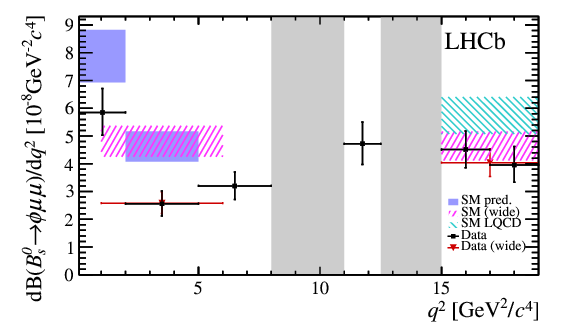
\includegraphics[width=0.7\textwidth]{figs_phimumu_branching}
  \caption{The figure shows the measured and predicted values for the
    differential branching ratio for $B_{s} \to \phi \mu\mu$ by bins of $q^{2}$.
    The data points are the LHC$b$ measurements, while the coloured rectangles
    are the SM predictions with form factors calculated using light-cone sum
    rules~\cite{Straub:2015ica, Altmannshofer:2014rta} and lattice
    QCD~\cite{Horgan:2013pva}. The greyed out regions correspond to charmonium
    resonances, exluded from the analysis as discussed in the main text. The
    LHC$b$ data points are generally lower than the SM expectation, especially
    in the $q^{2} \in [1, 5]~\GeV^{2}$ bin where the discrepancy is larger than
    $3\sigma$. The plot is taken from Ref.~\cite{Blake:2017wjz}.}
  \label{fig:phimumu_branching}
\end{figure}

The decay $B_{s} \to \mu \mu$ is cleaner than the semileptonic decays on the
theory side: the final state is leptonic and the only non-perturbative physics
needed is the $B_{s}$ decay constant, which can be calculated to high precision
on the lattice~\cite{Bobeth:2013uxa}. The measurements performed by
ATLAS~\cite{Aaboud:2018mst}, LHC$b$~\cite{Aaij:2012nna, Aaij:2017vad} and
CMS~\cite{CMS-PAS-BPH-16-004} are shown in Fig.~\ref{fig:Bsmumu_cms}, along with
correlated limits on $B^{0}\to \mu\mu$. The combination of the measurements
shown is taken from Ref.~\cite{Aebischer:2019mlg}, and suggests a compatibility
with the SM at close to $2\sigma$. Currently, measurements of $B_{s} \to \mu\mu$
are statistically limited; the branching ratio in the SM is very small because
it is chirality suppressed, but this also makes it a promising mode for
measuring new-physics effects.

\begin{figure}[t]
  \centering
  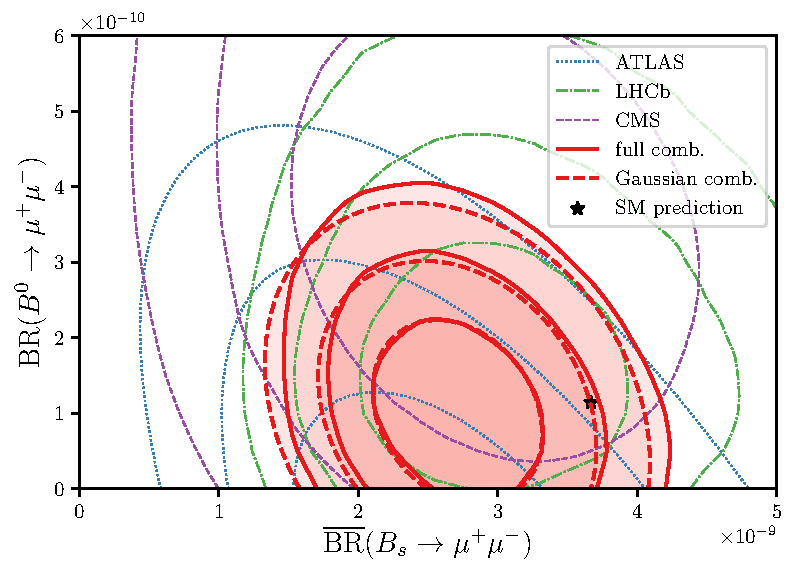
\includegraphics[width=0.7\textwidth]{Bsmumu}
  \caption{The figure shows the two-dimensional likelihood contours in
    $\mathrm{Br}(B^{0} \to \mu\mu)$ and $\mathrm{Br}(B_{s} \to \mu\mu)$. The
    thin contours are individual measurements, while the thick contours are the
    combination. A Gaussian approximation to the combined fit is shown with
    thick dashed contours. For more details see Ref.~\cite{Aebischer:2019mlg},
    from where the figure is taken. The SM prediction (shown with a star) is
    compatible with the combined fit at $2\sigma$.}
  \label{fig:Bsmumu_cms}
\end{figure}

The large theoretical uncertainties featuring in the expressions for the decay
rates $\Gamma[B\to K^{(*)} \mu\mu]$ can be tamed in a more direct way by
constructing a ratio with the electronic mode $B\to K^{(*)} ee$, in which many
sources of uncertainty cancel in the regime where new-physics effects are
small~\cite{Hiller:2003js, Capdevila:2017bsm, Capdevila:2016ivx}. Interestingly,
the LHC\textit{b} collaboration has measured a suppression in the ratios
\begin{equation}
  \label{eq:RK}
  R_{K^{(*)}} = \frac{\Gamma[B\to K^{(*)}\mu\mu]}{\Gamma[B\to K^{(*)} ee]}
\end{equation}
in the $q^{2} \in [1, 6]~\GeV^{2}$ bin. In the SM the prediction of the
observables outside of the low-$q^2$ region is determined by physics which is
wholly independent of the flavor of the lepton pair in the final state, making
$R_K$ and $R_{K^*}$ finely sensitive to violations of LFU. LHC\textit{b}
finds~\cite{Aaij:2019wad}
\begin{equation}
  \label{eq:RK2}
  R_K = 0.846\,_{-0.054-0.014}^{+0.060+0.016} \ ,
\end{equation}
for dilepton invariant mass squared range $q^2 \in [1.1, 6]~\GeV^{2}$, while the
SM demands $R^{\text{SM}}_K = 1.0003 \pm 0.0001$~\cite{Bobeth:2007dw}. The
analysis accounts for systematic differences in the reconstruction of muons and
electrons by LHC$b$ by first normalising the decay rates to the
$B^{+} \to K^{+} J/\psi (\to \mu\mu/ee)$ rates. The measurement is then a double
ratio in which many theoretical and experimental uncertainties cancel. The ratio
$R_{K}$ has also been measured by Belle~\cite{Abdesselam:2019lab} and BaBar~\cite{Lees:2012tva} to
be suppressed, although with larger uncertainties.

The $K^{*}$ ratio has also been measured by LHC\textit{b}~\cite{Aaij:2017vbb} to
show an approximately $2.5 \sigma$ discrepancy in the central $q^{2}$ bin:
\begin{equation}
  \label{eq:RKstar-lhcb}
    R_{K^*} = \begin{cases}
     0.660\,_{-0.070}^{+0.110}\pm 0.024 & \text{ for $\SI{0.045}{\GeV^{2}} < q^2 < \SI{1.1}{\GeV^{2}}$} \\
    0.685\,_{-0.069}^{+0.113}\pm 0.047 & \text{ for $\SI{1.1}{\GeV^{2}} < q^2 < \SI{6}{\GeV^{2}}$}
  \end{cases} \ .
\end{equation}
The Belle measurement~\cite{Abdesselam:2019wac} is consistent with the SM
prediction at $\lesssim 2\sigma$:
\begin{equation}
  \label{eq:RKstar-belle}
    R_{K^*} = \begin{cases}
     0.90\,_{-0.21}^{+0.27} \pm 0.10 & \text{ for $\SI{0.1}{\GeV^{2}} < q^2 < \SI{8}{\GeV^{2}}$} \\
    1.18\,_{-0.32}^{+0.52} \pm 0.10 & \text{ for $\SI{15}{\GeV^{2}} < q^2 < \SI{19}{\GeV^{2}}$}
  \end{cases} \ .
\end{equation}
Although the error bars are large, the central value is still suppressed with
respect to the SM prediction in the low-$q^{2}$ region. A summary of the
experimental situation relevant to $R_{K}$ and $R_{K^{*}}$ is presented in
Fig.~\ref{fig:rkrkstar-summary}.

\begin{figure}
  \centering
  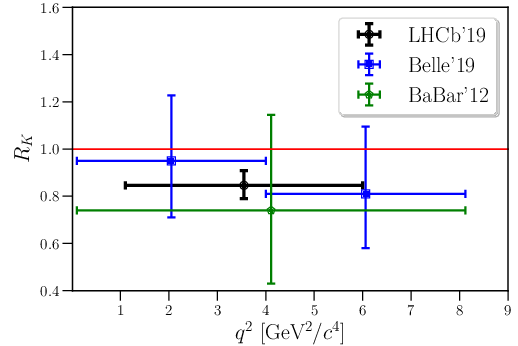
\includegraphics[width=0.7\textwidth]{RK-lowQ2}
  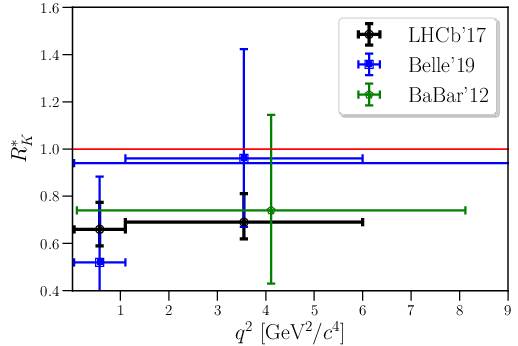
\includegraphics[width=0.7\textwidth]{RKstar-lowQ2}
  \caption{(top) The measurements of the LFU $R_{K}$ by
    LHC$b$~\cite{Aaij:2019wad}, Belle~\cite{Abdesselam:2019lab} and
    BaBar~\cite{Lees:2012tva}. All measurements are suppressed relative to the
    SM prediction, shown in red. (bottom) The figure shows the experimental
    situation for $R_{K^{*}}$~\cite{Lees:2012tva, Abdesselam:2019wac,
      Aaij:2017vbb}. Like $R_{K}$, the measured values are found to be smaller
    than the SM value, shown in red. Both figures are taken from
    Ref.~\cite{Koppenburg:2016rji}.}
  \label{fig:rkrkstar-summary}
\end{figure}

The distribution of final-state particles in the semileptonic decays
$B \to K^{*} \mu \mu$ define a number of angular observables, some of which have
also been measured to be in disagreement with SM predictions. The
$P_{5}^{\prime}$ asymmetry~\cite{Ali:1991is, Egede:2008uy,
  Descotes-Genon:2013vna} is constructed as a ratio of angular observables to
minimise from-factor uncertainties. Measurements show a significant deviation
from the SM at around $q^{2} \sim \SI{5}{\GeV^{2}}$~\cite{Aaij:2013qta,
  Aaij:2020nrf, Wehle:2016yoi, Aaboud:2018krd} as shown in
Fig.~\ref{fig:p5p-exp}, although the CMS measurement~\cite{Sirunyan:2017dhj} is
consistent with the SM prediction~\cite{Straub:2015ica, Altmannshofer:2014rta,
  Descotes-Genon:2014uoa, Khodjamirian:2010vf} in this region. The hadronic
uncertainties are still sizeable in this case.

\begin{figure}[t]
  \centering
  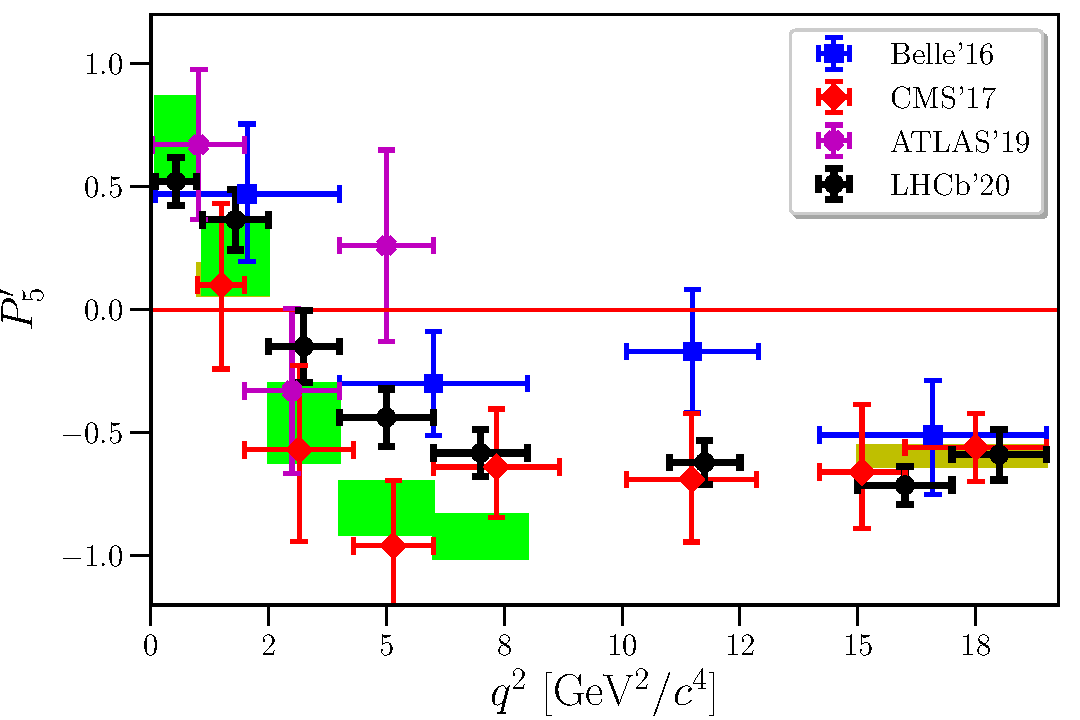
\includegraphics[width=0.7\textwidth]{P5prime}
  \caption{The figure shows the measured values of the $P_{5}^{\prime}$ angular
    observable in the decays $B \to K^{*} \mu\mu$ binned by $q^{2}$. With the
    exception of the CMS measurements, there is an enhancement with respect to
    the SM prediction (green) around $q^{2} \sim \SI{5}{\GeV^{2}}$. The plot is
    taken from Ref.~\cite{Koppenburg:2016rji}.}
  \label{fig:p5p-exp}
\end{figure}

\subsubsection{Fits}

The picture of the neutral-current anomalies given above is still only a small
cross-section of the several hundred observables that are in tension with the SM
predictions. A large number of global-fit analyses have been conducted in which
these anomalies are interpreted in terms of deviations in the operators $C_{9}$
and $C_{10}$, introduced above in Eq.~\eqref{eq:c9-c10}. These analyses are all
in mutual agreement, and generally find that a sizeable negative value for
$C_{9}$ is preferred over the SM value at between 4 and
$7\sigma$~\cite{Aebischer:2019mlg, Alguero:2019ptt, Arbey:2019duh,
  Ciuchini:2019usw}. (This was first pointed out in
Ref.~\cite{Descotes-Genon:2013wba}, which analysed the 2013 data.) This wide
range is largely due to differences in dealing with uncertainties in the
semileptonic decays. Importantly, no large deviation in the electronic modes is
necessary for a good fit. An example of one of the recent global
fits~\cite{Aebischer:2019mlg} to $C_{9}$ and $C_{10}$ is shown in
Fig.~\ref{fig:c9-c10-fit}. The authors find the single-operator best-fit
scenario to be in the $\mathrm{SU}_{L}(2)$-invariant direction
$C_{9} = -C_{10}$, with $C_{9} = -C_{10} = -0.53$ giving a pull from the SM of
$6.6\sigma$. We note that following the updated measurements of
$R_{K}$~\cite{Aaij:2019wad} and $R_{K^{*}}$~\cite{Abdesselam:2019wac} presented
at the 2019 Moriond conference, there is a slight tension between explaining the
LFU ratios and the rest of the $b\to s$ data. We point the reader to
Ref.~\cite{Aebischer:2019mlg} for a more detailed discussion on this point.

\begin{figure}[t]
  \centering
  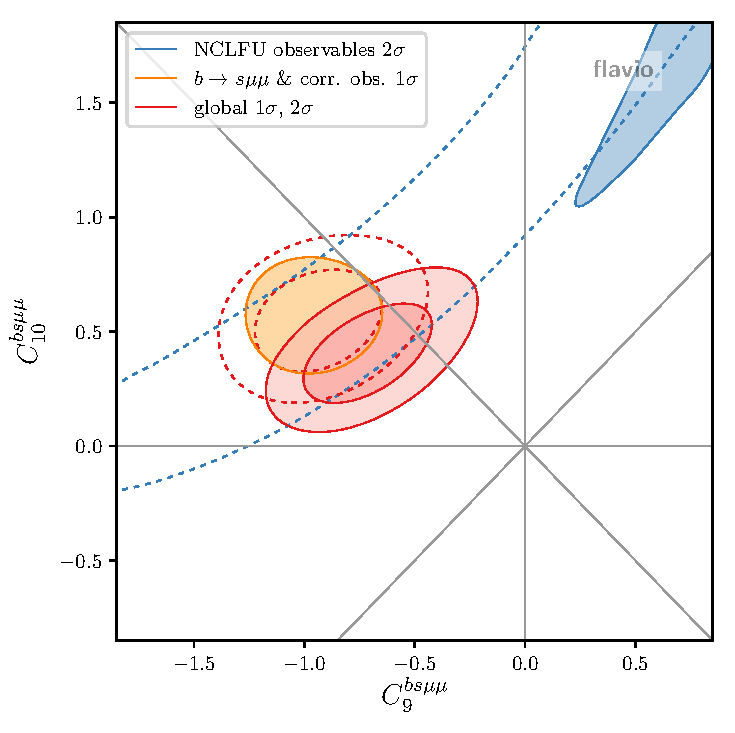
\includegraphics[width=0.7\textwidth]{bsmumu_C9_C10}
  \caption{The figure shows the results of the global fit conducted in
    Ref.~\cite{Aebischer:2019mlg} in the $C_{9}$--$C_{10}$ plane. The fit to
    just the LFU ratios is shown in blue, while that for the other $b\to s$ data
    is shown in yellow, with the combined fit shown in red. The
    $\mathrm{SU}(2)_{L}$-invariant direction $C_{9}=-C_{10}$ gives a good fit to
    the data, and any acceptible fit requires a sizeable negative value for
    $C_{9}$. The plot is taken from Ref.~\cite{Aebischer:2019mlg}.}
  \label{fig:c9-c10-fit}
\end{figure}

That much of the tension is driven by a deviation in $C_{9}$ also allows for an
explanation of many of the anomalies in a way that does not require the
introduction of new physics. The deviation in $C_{9}$ necessary to explain much
of the anomalous $b \to s$ data can be mimicked by non-perturbative effects
associated with loops of charm quarks, \textit{e.g.}~\cite{Blake:2017wjz}, and
the data seem to be currently consistent with both
hypotheses~\cite{Altmannshofer:2015sma, Descotes-Genon:2015uva}. Such effects
cannot account for the violation of LFU seen in the ratios $R_{K^{(*)}}$, again
highlighting their importance in understanding the potential role of new physics
in explaining the neutral-current anomalies.

\subsection{Charged-current anomalies}

The class of charged-current anomalies in the $b \to c$ transition consists of a
smaller number of measurements and processes. The primary observables of
interest are the LFU ratios
\begin{equation}
  \label{eq:1}
  R_{D^{(*)}} = \frac{\mathrm{Br}[B \to D^{(*)} \tau \nu]}{\mathrm{Br}[B \to D^{(*)} \ell \nu]} \ ,
\end{equation}
where $\ell$ denotes one of the light leptons: $\ell \in \{e, \mu\}$. The ratio
has been measured by BaBar~\cite{Lees:2012xj, Lees:2013uzd},
Belle~\cite{Huschle:2015rga, Hirose:2016wfn, Hirose:2017dxl, Abdesselam:2019dgh}
and LHC$b$~\cite{Aaij:2015yra, Aaij:2017uff, Aaij:2017deq}, with combined values
from HFLAV given by~\cite{Amhis:2019ckw}
\begin{equation}
  R_{D} = 0.340 \pm 0.027 \pm 0.013\quad \text{ and }\quad R_{D^{*}} = 0.295 \pm 0.011 \pm 0.008 \ .
\end{equation}
These combinations are in tension with the SM predictions~\cite{Bigi:2016mdz,
  Bernlochner:2017jka, Bigi:2017jbd, Jaiswal:2017rve} as averaged by HFLAV:
\begin{equation}
  R^{\text{SM}}_{D} = 0.299 \pm 0.003\quad \text{ and }\quad R^{\text{SM}}_{D^{*}} = 0.258 \pm 0.005
\end{equation}
at approximately $3\sigma$. We note that BaBar and Belle use the average of the
electronic and muonic modes in the denominator, while LHC$b$ uses only the
muonic mode. The tension was significantly decreased following the most recent
Belle measurement presented at the Moriond 2019
conference~\cite{Abdesselam:2019dgh}; this combined measurement is consistent
with the SM prediction at $1.2\sigma$. A summary of the measurements of
$R_{D^{(*)}}$ is shown in Fig.~\ref{fig:rd-rdstar-hflav}.
BaBar~\cite{Lees:2013uzd} and Belle~\cite{Huschle:2015rga} have measured the
$q^{2}$ distributions of the tau-mode decay rate, which has proved to be a
powerful model discriminator, \textit{e.g.}~\cite{Freytsis:2015qca}.

\begin{figure}[t]
  \centering
  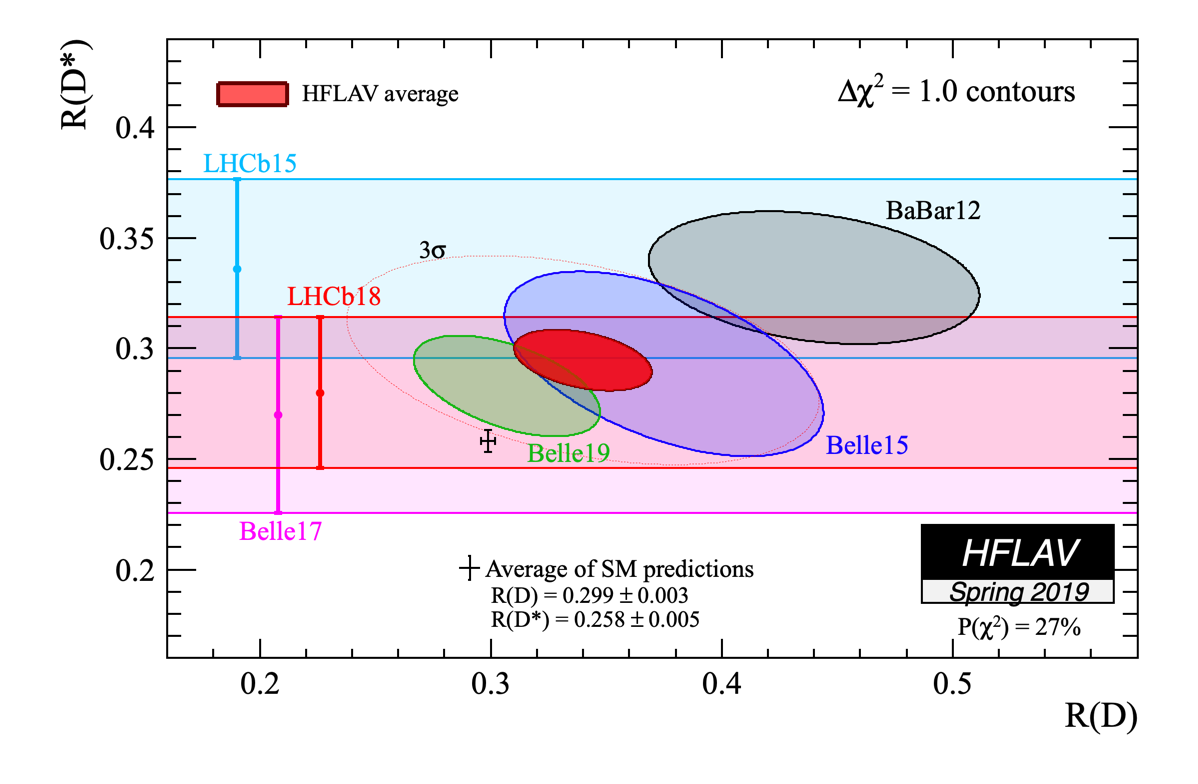
\includegraphics[width=0.9\textwidth]{rdrds_spring2019}
  \caption{The figure shows the combined fit to the available $R_{D}$ and
    $R_{D^{*}}$ data from HFLAV~\cite{Amhis:2019ckw}. The combination is shown
    in red, just over $3\sigma$ away from the SM prediction (black data point).
    Both ratios are measured to be enhanced compared to the SM value.}
  \label{fig:rd-rdstar-hflav}
\end{figure}

Although the ratios $R_{D^{(*)}}$ are our primary concern in this work, we also
introduce a number of other observables relevant to the charged current process.
The first of these is the LFU ratio $R_{J/\psi}$:
\begin{equation}
  \label{eq:rjpsi}
  R_{J/\psi} = \frac{\mathrm{Br}(B_{c} \to J/\psi \tau \nu)}{\mathrm{Br}(B_{c} \to J/\psi \mu \nu)} \ ,
\end{equation}
has recently been measured by LHC$b$ to be
$R_{J/\psi} = 0.71 \pm 0.17 \pm 0.18$~\cite{Aaij:2017tyk}. Although the ratio is
also measured to be enhanced with respect to the SM prediction
$R_{J/\psi}^{\text{SM}} \approx 0.25$--$0.29$~\cite{Anisimov:1998uk,
  Kiselev:2002vz, Ivanov:2006ni, Hernandez:2006gt, Huang:2007kb, Wang:2008xt,
  Issadykov:2018myx, Wen-Fei:2013uea, Alok:2017qsi, Azatov:2018knx, Hu:2019qcn,
  Leljak:2019eyw, Azizi:2019aaf}, the central value of the measurement shows a
very large effect that cannot be well-accommodated with BSM
contributions~\cite{Murgui:2019czp}, although the error bars are very large. The
observable $f_L^{D^*}$, the longitudinal polarisation of the $D^*$ in
$B \to D^* \tau \nu$, also differs from the SM expectation by $\sim 1.6 \sigma$:
\begin{equation}
    f_L^{D^*} = 0.60 \pm 0.08 \pm 0.04,
\end{equation}
as measured by the Belle collaboration~\cite{Abdesselam:2019wbt}, and has been
shown to have good discriminating power for BSM explanations of $R_{D^{(*)}}$.
The third class of observables we consider are tau polarisation asymmetries [see
Ref.~\cite{Asadi:2018sym} for a detailed discussion in the context of explaining
$R_{D^{(*)}}$]. The polarisation asymmetry in the longitudinal direction of the
$\tau$ in the $D^*$ mode has also recently been measured by
Belle~\cite{Hirose:2016wfn}:
\begin{equation}
\mathcal{P}_{\tau}^{*} = -0.38 \pm 0.51^{+0.21}_{-0.16} .
\end{equation}
Although the errors are large, the projected Belle II sensitivity at
$50 \text{ ab}^{-1}$ for the same observable in the $D$ mode is estimated at
about $3\%$~\cite{Alonso:2017ktd}, and we expect the $\mathcal{P}_\tau^{*}$ to
be measured even more precisely at Belle II.

The leptonic decays of the charmed $B$ meson have not been measured yet,
although measurements of its lifetime may imply serious constraints on models
attempting to explain the discrepancies in $R_{D}$ and $R_{D^{*}}$ with new
physics. A number of groups have inferred a wide variety of limits
\begin{equation}
  \label{eq:bctaunu-limits}
 \mathrm{Br}(B_{c} \to \tau \nu) < [0.1, 0.6]
\end{equation}
using differing theoretical arguments~\cite{Li:2016vvp, Akeroyd:2017mhr,
  Alonso:2016oyd, Blanke:2018yud, Bardhan:2019ljo}. The range of limits is so
wide because it is sensitive to the ratio of hadronisation probabilities of the
charm and up quarks: $f_{c}/f_{u}$. The range of values given for the limit in
Eq.~\eqref{eq:bctaunu-limits} corresponds only to a change in $f_{c}/f_{u}$ of a
factor of five~\cite{Bardhan:2019ljo}.

{\color{red} John, When you put in chapter 3, move discussion of agreement in
  LFU between light-lepton modes and absence of lattice results for
  $B \to D^{*}$ form factors here.}

\subsubsection{Fits}

The charged-current $b \to c$ anomalies can be interpreted in terms of
deviations from dimension-six operator coefficients in the WET. The pertinent
Hamiltonian for $b \to c \ell_{r} \nu_{s}$ is
\begin{equation}
  \label{eq:bctaunu-ham}
  H^{b\to c}_{\text{eff}} = \frac{4 G_{F}}{\sqrt{2}} V_{cb} \sum_{rs} [(\delta^{rs} + C^{rs}_{V_{L}}) \mathcal{O}^{rs}_{V_{L}} + C_{V_{R}}^{rs} \mathcal{O}^{rs}_{V_{R}} + C^{rs}_{S_{L}}\mathcal{O}^{rs}_{S_{L}} + C^{rs}_{S_{R}}\mathcal{O}^{rs}_{S_{R}} + C^{rs}_{T}\mathcal{O}^{rs}_{T}] + \text{h.c.}
\end{equation}
where
\begin{equation}
    \mathcal{O}^{rs}_{V_{X}} = (\bar{c} \gamma^{\mu} P_{X} b) (\bar{e}_{r} \gamma_{\mu} P_{L} \nu_{s}) \ , \, \mathcal{O}^{rs}_{S_{X}} = (\bar{c} P_{X} b) (\bar{e}_{r} P_{L} \nu_{s}) \ , \, \mathcal{O}^{rs}_{T} = (\bar{c} \sigma^{\mu\nu} P_{X} b) (\bar{e}_{r} \sigma_{\mu\nu} P_{L} \nu_{s}) \ ,
\end{equation}
and $X \in \{L, R\}$. The left-handed vector operator is the same one generated
in the SM, while the scalar and tensor operators can provide large enhancements
to the decay rate, since they lift the helicity-suppression.

A number of analyses have considered interpreting the measurements of $R_{D}$
and $R_{D^{*}}$ in the context of these operators, usually restricting to
single-operator fits, \textit{e.g.}~\cite{Sakaki:2013bfa, Freytsis:2015qca,
  Jung:2018lfu, Azatov:2018knx, Angelescu:2018tyl, Huang:2018nnq,
  Murgui:2019czp}. In Fig.~\ref{fig:rd-rdstar-fit} we present a plot taken from
Ref.~\cite{Murgui:2019czp} in which the effects of each of the operators on the
observables of interest are explored. The plot indicates that a number of
single-operator solutions exist that reconcile the predicted and measured values
for both $R_{D}$ and $R_{D^{*}}$, although single-operator resolutions of the
mild tension in $f_{L}^{D^{*}}$ are disfavoured by the limits on the $B_{c}$
lifetime, discussed above.

\begin{figure}
\centering
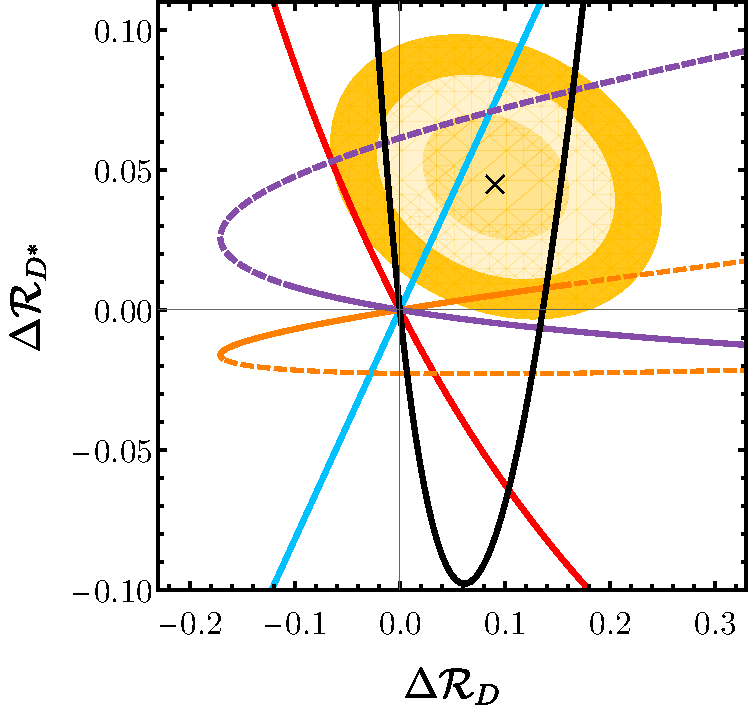
\includegraphics[scale=0.5]{RDvsRDstar_vN.pdf}
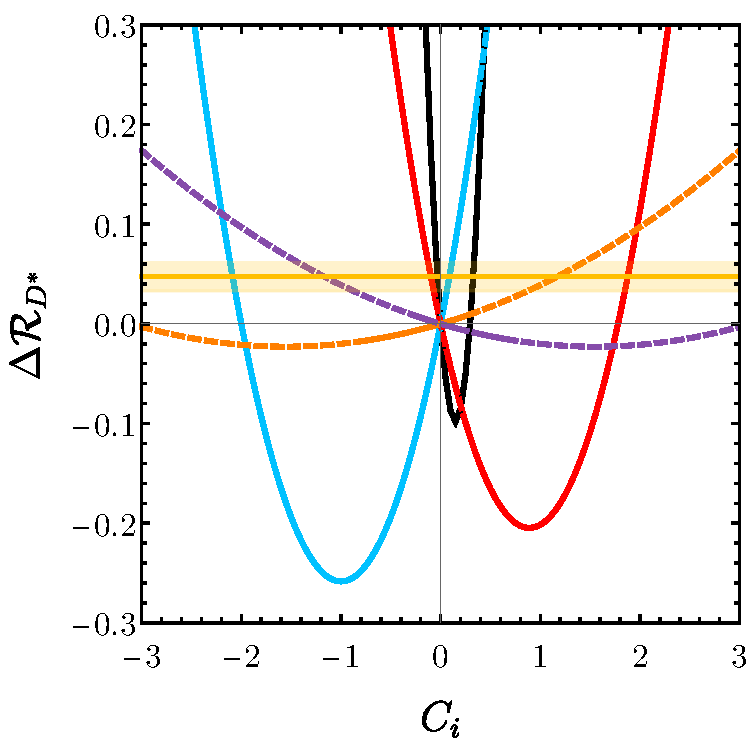
\includegraphics[scale=0.5]{RDstarvsCi.pdf}
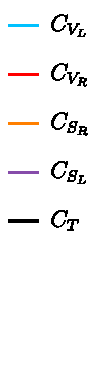
\includegraphics[scale=0.9]{LegendCi.pdf}
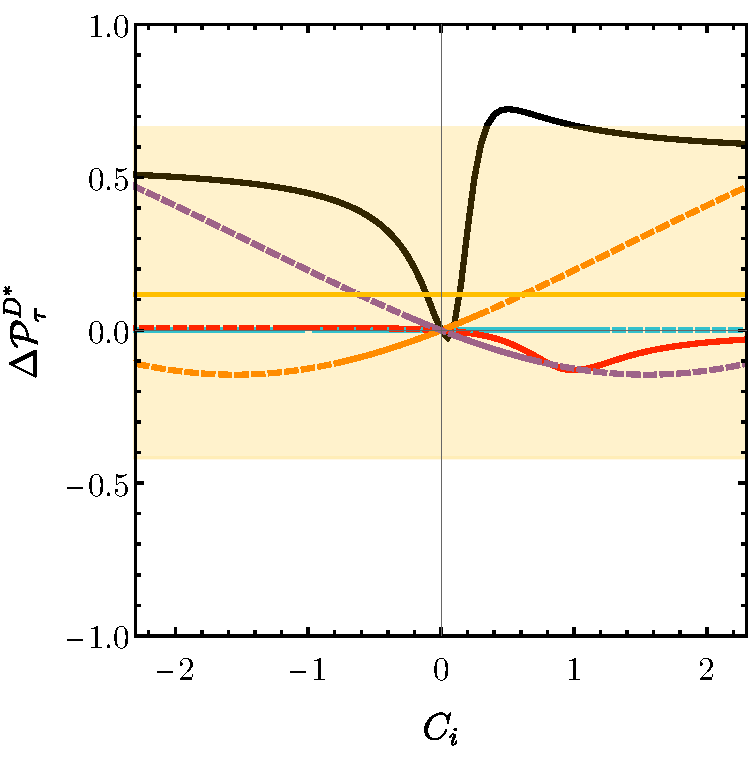
\includegraphics[scale=0.5]{PDstarvsCi_vN.pdf}
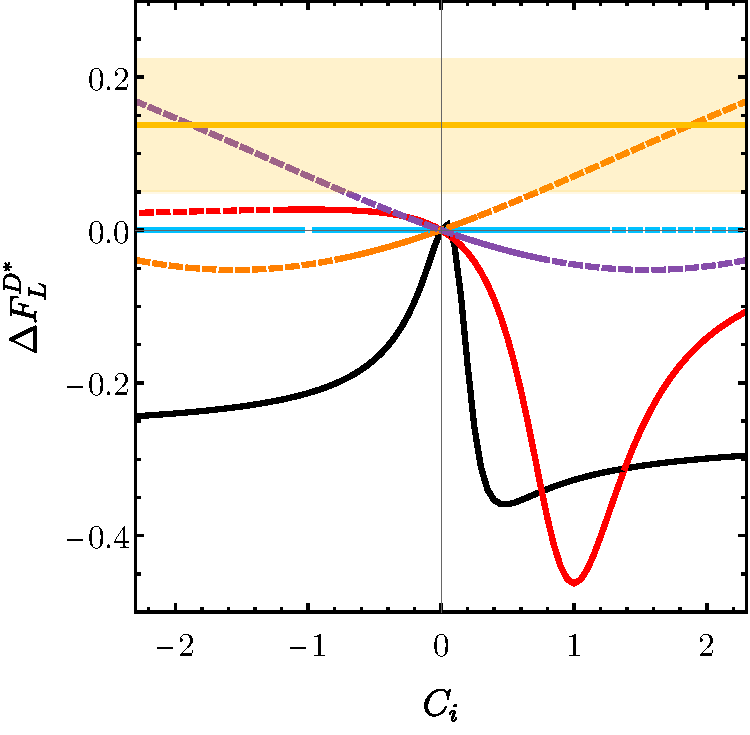
\includegraphics[scale=0.5]{FLDstarvsCi_vN.pdf}
\phantom{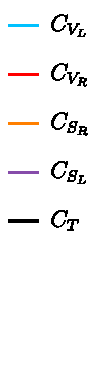
\includegraphics[width=0.09\linewidth]{LegendCi.pdf}}
\caption{Individual contributions of the Wilson coefficients of the WET
  Hamiltonian in different observables ($\Delta X \equiv X-X_{\text{SM}}$):
  correlation between $\Delta {\cal R}_D$ and $\Delta {\cal R}_{D^*}$, and
  $\Delta \mathcal{R}_{D^*}$, $\Delta \mathcal{P}_\tau^{D^{*}}$ and
  $\Delta {\cal F}_L^{D^{*}}$ as a function of the Wilson coefficients. Left-top
  panel: the experimental central value is denoted by a black cross and the
  $1\sigma, 2\sigma$ and $3\sigma$ uncertainties by yellow rings. Right-top and
  bottom panels: experimental central values are displayed by a solid yellow
  line and their $1\sigma$ uncertainty by a yellow band. Dashed lines indicate
  regions excluded by the constraint $\mathrm{Br}(B_c \to \tau \nu) < 0.1$.}
\label{fig:rd-rdstar-fit}
\end{figure}

\subsection{Anomalous magnetic moment of the muon}

The most precise measurement of the anomalous magnetic moment of the muon
\begin{equation}
  a_{\mu} \equiv \frac{(g-2)_{\mu}}{2}
\end{equation}
shows a sizeable tension with the SM prediction. The difference between the
measured value~\cite{Chapelain:2017syu, Blum:2013xva} and the SM prediction~\cite{} is
\begin{equation}
\Delta a_\mu= a_\mu^{\text{exp}} - a_\mu^{\text{SM}}= (286 \pm 63 \pm 43) \cdot 10^{-11} \ ,
\end{equation}
corresponding to a $3.6\sigma$ discrepancy. More recently, the measured value
$a_{e}$, the anomalous magnetic moment of the electron, has also been found to
disagree with the SM value at $2.5\sigma$~\cite{articleParker}.


\myglossaryentry{lipsum}{lipsum}{Lorem Ipsum, a special type of fudge}{}
\myglossaryentry{dolor}{dolor}{No idea why}{parent={lipsum}}
\myglossaryentry{ibit}{ibit}{Sounds right, doesn't it?}{parent={lipsum}}
\myacronym{DFT}{density functional theory}
\myglossaryentry{$\pi$}{pi}{Greek letter pi, \ensuremath{\Pi} does this work?}{symbol={$\pi$}}
\myacronym{RDF}{radial distribution function}
\myglossaryentry{radial distribution function}{radialdistributionfunction}{}{symbol={$g(r)$}}
